
%%%%%%%%%%%%%%%%%%%%%%%%%%%%%%%%%%%%%%%%%%%%%%%%%%%%%%%

\documentclass{iitthesis}
%\documentclass[draft]{iitthesis}

% Document Options:
%
% Note if you want to save paper when printing drafts,
% replace the above line by
%
%   \documentclass[draft]{iitthesis}
%
% See Help file for more about options.

\usepackage[dvips]{graphicx}    % This package is used for Figures
\usepackage{rotating}           % This package is used for landscape mode.
\usepackage{epsfig}
\usepackage{subfigure}          % These two packages, epsfig and subfigure, are used for creating subplots.
% Packages are explained in the Help document.
\usepackage{amsmath,amssymb,amsthm,mathtools,bbm,booktabs,array,tikz,pifont,comment,multirow,url,graphicx}
\usepackage{enumitem}
\usepackage[nodayofweek]{datetime}
\usepackage{color}
\input FJHDef.tex

%Requires ApproxUnivariate_k.tex, univariate_integration_k.tex, ConesPaperSpikyquad.eps, ConesPaperFlukyquad.eps

\DeclareMathOperator{\Var}{Var}
\DeclareMathOperator{\INT}{INT}
\DeclareMathOperator{\APP}{APP}
\DeclareMathOperator{\lin}{lin}
\DeclareMathOperator{\up}{up}
\DeclareMathOperator{\lo}{lo}
\DeclareMathOperator{\fix}{fix}
\DeclareMathOperator{\err}{err}
\DeclareMathOperator{\maxcost}{maxcost}
\DeclareMathOperator{\mincost}{mincost}
\newcommand{\herr}{\widehat{\err}}

\newtheorem{theorem}{Theorem}
\newtheorem{prop}[theorem]{Proposition}
\newtheorem{lem}{Lemma}
\newtheorem{cor}{Corollary}
\theoremstyle{definition}
\newtheorem{algo}{Algorithm}
\newtheorem{condit}{Condition}
%\newtheorem{assump}{Assumption}
\theoremstyle{remark}
\newtheorem{rem}{Remark}
\newcommand{\Fnorm}[1]{\abs{#1}_{\cf}}
\newcommand{\Ftnorm}[1]{\abs{#1}_{\tcf}}
\newcommand{\Gnorm}[1]{\norm[\cg]{#1}}
\newcommand{\flin}{f_{\text{\rm{lin}}}}
%\newcommand{\dif}{\textup{d}}

\begin{document}

%%% Declarations for Title Page %%%
\title{Guaranteed, Adaptive, Automatic Algorithms for Univariate Integration: Methods, Cost, and Implementations}
\author{Yizhi Zhang}
\degree{Doctor of Philosophy}
\dept{Applied Mathematics}
\date{\today}
\copyrightnoticefalse      % crate copyright page or not
%\coadvisortrue           % add co-advisor. activate it by removing % symbol to add co-advisor
\maketitle                % create title and copyright pages


\prelimpages         % Settings of preliminary pages are done with \prelimpages command


%%%  Acknowledgement %%%
\begin{acknowledgement}     % acknowledgement environment, this is optional
\par  Will be added once thesis is finished
% or \input{acknowledgement.tex} % you need a separate acknowledgement.tex file to include it.
\end{acknowledgement}


% Table of Contents
\tableofcontents
\clearpage

% List of Tables
\listoftables

\clearpage

%List of Figures
\listoffigures

\clearpage

%List of Symbols(optional)

\listofsymbols
 \SymbolDefinition{$\beta$}{List of symbols will be added later}

 \clearpage



%%% Abstract %%%
\begin{abstract}           % abstract environment, this is optional
\par Abstract will be included once all parts are finished
% Those algorithms will be firstly created based on the composite trapezoidal rule. It is the "simplest??"
% or  This thesis investigates how to solve univariate integration problems using numerical methods, including the trapezoidal rule and the Simpson's rule. Most existing guaranteed algorithms are not adaptive and require too much a priori information. Most existing adaptive algorithms do not have valid justification for their results. The goal is to create adaptive algorithms utilizing the two above-mentioned methods with guarantees. The classes of integrands studied in this thesis are cones. The algorithms are analytically proved to be a success if the integrand lies in the cone. The algorithms are adaptive and automatically adjust the computational costs based on the integrand values. The lower and upper bounds on the computational costs for both algorithms are derived. The lower bounds on the complexity of the problems are derived as well. By comparing the upper bounds on the computational cost and the lower bounds on the complexity, our algorithms are shown to be asymptotically optimal. Numerical experiments are implemented.   %you need a separate abstract.tex file to include it.
\end{abstract}


\textpages     % Settings of text-pages are done with \textpages command

% Chapters are created with \Chapter{title} command
\Chapter{Introduction}
%\section{Numerical Integration and Applications}

In numerical analysis, numerical integration plays an important role. It uses a certain algorithm to calculate the numerical value of a definite integral. It is used instead of those general and mathematically sophisticated analytical methods because that sometimes the problem is lack of analytical solution, or the integrand is only known at certain points by sampling. In this thesis, we will focus on the univariate integration problem
\begin{equation}\label{integral}
    \text{INT}(f)=\int_{a}^{b}f(x)\,\textup{d}x\in\reals.
\end{equation}
We will provide two adaptive automatic algorithms, $\text{integral}\_\text{t}$, and $\text{integral}\_\text{s}$, that use trapezoidal rule and Simpson's rule respectively, and are guaranteed to provide numerical approximations no differ from the true integral by a specified error tolerance $\varepsilon$, i.e.
\begin{align}\label{approx}
      \left|\int_{a}^{b}f(x)\,\textup{d}x-\text{integral}\_\text{t}(f,\varepsilon)\right|\leq \varepsilon,& \\
      \left|\int_{a}^{b}f(x)\,\textup{d}x-\text{integral}\_\text{s}(f,\varepsilon)\right|\leq \varepsilon,&
\end{align}
assuming that $\forall f \in \cc^{p}, a,b\in\reals, a<b, \varepsilon>0$, where $a$ and $b$ are finite, and $\cc^{p}$ are some sets of integrands defined in the later part of the thesis.

%adaptively determine the computational cost required to obtain a result of the integral. The required inputs are both an error tolerance, $\varepsilon$, %and the integrand $f$. The output will be guaranteed to not differ from the true answer by more than $\varepsilon$.
Our algorithms are adaptive. By adaptive, it means that the algorithms automatically expand the right amount of computational effort needed to provide an approximate solution within the error tolerance. Our algorithms are also guaranteed to satisfy the error tolerance. Other existing guaranteed algorithms are usually not adaptive. They cannot adjust their effort based on the property of the input function. Details about those algorithms are discussed in section \ref{secgua}.

The essence of every adaptive algorithm is an error estimate of the numerical approximation based on the computations already performed. For those existing adaptive algorithms, these error estimates either require too much information from the user or based on heuristics and not guaranteed. Details about those algorithms are discussed in section \ref{secada}.

\Section{Fixed-Cost Algorithms for Balls of Input Functions}\label{secgua}

Fixed-cost algorithms with guarantees usually require input functions to lying in a ball-shaped function space. Traditional trapezoidal rule and Simpson's rule in calculus courses are two typical examples of fixed-cost algorithms. They have upper bounds on approximation error in terms of the total variation of a particular derivative of integrand:
\begin{align}\label{errorsimple}
    \text{err}(f,n)\le\overline{\text{err}}(f,n):=&C(n)\Var(f^{(p)}),
\end{align}
for trapezoidal rule, $p=1$; for Simpson's rule, $p=3$. In order to make sure that the algorithms succeed, users need to obtain information about the total variation of the integrand. So the algorithms only provide guarantees when the total variation has an upper bound, namely $\Var(f^{p})<\sigma$. The computational cost $n=C^{-1}(\varepsilon/\sigma)$. Those algorithms are automatic because it the computational effort required is depended on the error tolerance.

Those algorithms have drawbacks. Firstly, users may not obtain the properties of the input function. If a moderate $\sigma$ is selected. The algorithms may work for easy functions but not for functions with sharp peaks. Secondly, if the algorithms work for $f$, it may not work for $cf$, where $c$ is a constant and $c>1$, because $cf$ may fall out of the ball. Moreover, those algorithms have the computational cost depending on $\sigma$, which does not depend on function values. Thus, those functions are not adaptive.

\Section{Adaptive Algorithms with No Guarantees}\label{secada}

Adaptive, automatic algorithms are commonly used in numerical software packages. MATLAB's integral and Chebfun are two well-known examples. These methods do not require a value of $\sigma$. Instead, they estimate the error using only function values and then determine the sample size accordingly. These algorithms work well in many cases. However, they do not have rigorous justification. Namely, one cannot tell whether the answer provided by the algorithm is true or not. Therefore, the asymptotic error estimates from these algorithms are heuristics and do not hold for all cases. Users can always fool these methods by giving them a peak-shaped function with the width less than the mesh size. In this case, the algorithms cannot detect the peak and return zero as an answer.

In fact, the challenge of spiky integrands applies to algorithm that depends on function values, including ours. In contrast to fixed-cost algorithms, our methods are adaptive and succeed for a cone of integrands. In contrast to the adaptive algorithms, our methods have rigorous proof of how spiky an integrand can be to stay inside the cone.






\Section{Motivation and Outline}

The goal is to construct adaptive, automatic algorithms with guarantees of success. In Chapter 2, we introduce the definitions and assumptions used in the thesis. Chapter 3 will focus on finding upper bound on approximation error and rigorous theoretical proof of success. Guaranteed algorithms are presented in Chapter 4 with the lower and upper bound of the computational cost. Chapter 5 studies the lower bound of complexity. In Chapter 6, the results from numerical experiences will be discussed.  The guaranteed algorithms derived here are based on trapezoidal rule and Simpson's rule. The former is simple but has a lower order of convergence rate The latter has a higher convergence rate but the derivation is more complicated. The derivation of the two algorithms is done in parallel in Chapters 4 to 6 for the trapezoidal rule and Simpson's rule.

\clearpage



\Chapter{Problem Statement and Assumptions}


The previous chapter introduced the univariate integration problem. The building blocks of the adaptive, automatic algorithms are two widely used fixed cost algorithms, trapezoidal rule and Simpson's rule.
The composite trapezoidal rule can be defined as:
\begin{equation}\label{traprule}
  T(f,n)=\frac{b-a}{2n}\sum_{j=0}^{n}(f(u_{j})+f(u_{j+1})),
\end{equation}
where
\begin{equation}\label{upts}
u_j=a+\frac{j(b-a)}{n}, \qquad j=0, \ldots, n, \qquad n\in\mathbb{N}.
\end{equation}
It uses $n+1$ function values where those $n+1$ node points are equally spaced between $a$ and $b$. The composite Simpson's rule can be defined as:
\begin{equation}\label{simrule}
  S(f,n)=\frac{b-a}{18n}\sum_{j=0}^{3n-1}(f(v_{2j})+4f(v_{2j+1})+f(v_{2j+2})),
\end{equation}
where
\begin{equation}\label{vpts}
v_j=a+\frac{j(b-a)}{6n}, \qquad j=0, \ldots, 6n, \qquad n\in \naturals.
\end{equation}
It uses $6n+1$ equally spaced function values, which form $6n$ intervals/subintervals between $a$ and $b$. The reason why we use $6n$ intervals is that firstly, Simpson's rule requires an even number of intervals. Secondly, we are going to use a third order finite difference to approximate the third derivative of $f$ in later chapters. This third order finite difference method requires the number of intervals to be a multiple of 3. Thus, the number of intervals for input data has to be a multiple of 6.

% Finding a proper way to approximate the first and third order derivatives plays an important role in constructing our algorithms, especially in finding the upper bound of approximation error.
We also need to find error bounds to guarantee our methods. Traditional non-adaptive trapezoidal rule and Simpson's rule have upper bounds on approximation error in terms of the total variation of a particular derivative of integrand as mentioned in \eqref{errorsimple}. Here we give detailed definitions on $C(n)$:
\begin{align}\label{errorbound}
    \text{err}(f,n)\le\overline{\text{err}}(f,n):=&C(n)\Var(f^{(p)}),\\
    \nonumber&C(n)=
    \begin{cases*}
           \frac{(b-a)^2}{8n^2}, p=1,  & \mbox{trapezoidal rule}\cite[(7.15)]{BraPet11a}, \\
           \frac{(b-a)^4}{5832n^4}, p=3, & \mbox{Simpson's rule}.
    \end{cases*}
\end{align}
check 5832 add ref.

To define the total variation, $\Var(f)$, firstly we introduce $\widehat{V}(f,\{x_i\}_{i=0}^{n+1})$ as an under-approximation of the total variation:
\begin{equation}\label{defvhat}
    \widehat{V}(f,\{x_i\}_{i=0}^{n+1})=\sum_{i=1}^{n-1}|f(x_{i+1})-f(x_{i})|,
\end{equation}
where $\{x_i\}_{i=0}^{n+1}$ is any partition with not necessarily equal spacing, and $a=x_{0}\leq x_{1}<\cdots<x_{n}\leq x_{n+1}=b$.
We use $n+2$ points and ignore $x_0$ and $x_{n+1}$ in \eqref{defvhat} for convenience later.
The total variation can be defined as the upper of bound on $\widehat{V}(f,\{x_i\}_{i=0}^{n+1})$:
\begin{equation}\label{defvar}
  \Var(f) := \sup \left\{\widehat{V}(f,\{x_i\}_{i=0}^{n+1}), \quad \text{for any }n \in \naturals, \text{ and } \{x_i\}_{i=0}^{n+1}\right\}.
\end{equation}
To ensure a finite error bound, our algorithms are defined for function spaces with finite total variations of the respective derivatives:
\begin{equation}\label{defspace}
 \cv^{p}:=\{f\in C[a,b]: \Var(f^{(p)}) < \infty \},
\end{equation}
where for trapezoidal rule, $p=1$, and for Simpson's rule, $p=3$.

Our algorithms will not work for all $f \in \cv^{p}$ because $f$ may have changes in $f^{(p)}$ on small intervals that the algorithms cannot detect. In order to build adaptive automatic and guaranteed algorithms, we set up the following assumptions that all functions to be integrated must lie in a cone of integrands for which $\widehat{V}(f^{(p)},\{x_i\}_{i=0}^{n+1})$ does not underestimate $\Var(f^{(p)})$ too much:
\begin{multline}\label{defcone}
\cc^{p}:=\left\{f\in \cv^{p}, \Var(f^{(p)})\leq \mathfrak{C}(\text{size}(\{x_i\}_{i=0}^{n+1}))\widehat{V}(f^{(p)},\{x_i\}_{i=0}^{n+1}),\right.\\ \left.\text{for all choices of } n\in \mathbb{N}, \text{and }\{x_i\}_{i=0}^{n+1} \text{ with }\text{size}(\{x_i\}_{i=0}^{n+1})<\mathfrak{h}\right\}.
\end{multline}
The cone space $\cc^{p}$ is a subset of $\cv^{p}$. Here $\text{size}(\{x_i\}_{i=0}^{n+1})$ is the largest possible width between any adjacent $x_i$:
\begin{equation}\label{defsize}
  \text{size}(\{x_i\}_{i=0}^{n+1}):=\max_{i=0,\cdots, n} x_{i+1}-x_{i}.
\end{equation}
The cut-off value $\mathfrak{h} \in (0, b-a)$ and the inflation factor $\mathfrak{C}: [0,\mathfrak{h} \rightarrow [1.\infty)$ define the cone. The choice of $\mathfrak{C}$ is flexible, but it must be non-decreaing. In this thesis, we choose
\begin{equation}\label{definflationfactor}
  \mathfrak{C}(h):=\frac{\mathfrak{C}(0)}{1-h/\mathfrak{h}}; \quad \mathfrak{C}(0)>1
\end{equation}
for convenience.

With the cone space defined, we can start constructing our adaptive trapezoidal rule and Simpson's rule algorithms for functions in $\cc^{p}$, with appropriate value of $p$. To begin with, Chapter 3 will show how the algorithms confidently estimate the error and provide data-driven error bounds.




\Chapter{Data-Driven Error Bound}

In this chapter, we will derive upper bounds with quadrature error in terms of function values. By \eqref{errorbound} in Chapter 2, we know that the approximation errors of trapezoidal rule and Simpson's rule have an upper bound in terms of the total variation of the appropriate derivatives. The definition of the cone suggests a way of bounding $\Var(f^{(p)})$ in terms of $\widehat{V}(f^{(p)},\{x_i\}_{i=0}^{n+1})$. However, our algorithms are based on function values and $\widehat{V}(f^{(p)},\{x_i\}_{i=0}^{n+1})$ is defined in terms of derivative values. Thus we will use finite differences to express derivative values in terms of function values.

\Section{Trapezoidal Rule}

We used the backward finite difference to approximate $f'$. Let $h=u_{j+1}-u_{j}=(b-a)/n$ and
\begin{align*}
  f[u_{j}]&=f(u_{j}), \text{ for } j=0,\cdots, n,\\
  f[u_{j},u_{j-1}]&=\frac{f(u_{j})-f(u_{j-1})}{h},\text{ for } j=1, \cdots, n.
\end{align*}


According to Mean Value Theorem for finite differences, (ref), for all $j=1,2,\cdots,n$, there exists $x_j\in (u_{j-1},u_{j})$ such that
\begin{equation*}
   f'(x_j)= f[u_{j},u_{j-1}],
\end{equation*}
for $j = 1, 2, \cdots, n.$ This implies that
\begin{equation}\label{fprime}
  f'(x_j)=\frac{f(u_{j})-f(u_{j-1})}{h}=\frac{n}{b-a}[f(u_{j})-f(u_{j-1})],
\end{equation}
for some $x_j\in (u_{j-1},u_{j})$. Let $\{a=x_{0}, x_{1},\cdots,x_{n},x_{n+1}=b\}$ be a partition as was introduced just below \eqref{defvhat}. Note that no matter how the $x_j$'s are located, the largest possible width cannot be larger than two intervals. So
\begin{equation}\label{cutoff1}
  \text{size}(\{x_j\}_{j=0}^{n+1})\leq 2h=2(b-a)/n<\mathfrak{h}.
\end{equation}
Since \eqref{defvhat} is true for all partition $\{x_i\}_{i=0}^{n+1}$, it is true for \eqref{fprime} with this particular partition $\{x_j\}_{i=0}^{n+1}$. Then we have the approximation $\widetilde{V}_1(f,n)$ to $\widehat{V}(f^{(p)},\{x_j\}_{i=0}^{n+1})$ using only function values:
\begin{align}\label{vtilde1}
\nonumber    \widehat{V}(f',\{x_j\}_{j=0}^{n+1})&= \sum_{j=1}^{n-1}\left|f'(x_{j+1})-f'(x_{j})\right|,\\
\nonumber    &=\sum_{j=1}^{n-1}\left|\frac{n}{b-a}[f(u_{j+1})-f(u_{j})-f(u_{j})+f(u_{j-1})]\right|\\
    &=\frac{n}{b-a}\sum_{j=1}^{n-1}\left|f(u_{j+1})-2f(u_{j})+f(u_{j-1})\right|=:\widetilde{V}_1(f,n).
\end{align}

Therefore by combining the deduction above together, we obtain the error bound for our trapezoidal rule algorithm using only function values:
\begin{align*}
\overline{\text{err}}(f,n):=&C(n)\Var(f'),\qquad &\text{ (by \eqref{errorbound})}\\
\leq & C(n)\mathfrak{C}(\text{size}(\{x_i\}_{i=0}^{n+1}))\widehat{V}(f',\{x_i\}_{i=0}^{n+1}), \qquad &\text{ (by \eqref{defcone})}\\
=& C(n)\mathfrak{C}(\text{size}(\{x_j\}_{i=0}^{n+1}))\widetilde{V}_1(f,n), \qquad &\text{ (by \eqref{vtilde1})}\\
  \leq & \frac{(b-a)^2\mathfrak{C}(2(b-a)/n)\widetilde{V}_1(f,n)}{8n^2}.\qquad &\text{ (by \eqref{cutoff1})}
\end{align*}

Thus, we have the following lemma.
\begin{lem}\label{lemmaerrorboundtrap}
    The approximation error of the composite trapezoidal rule is bounded in term of the function values of the input function as follows:
    \begin{equation}\label{errortrapcone}
      \overline{\textup{err}}_{\text{t}}(f,n)\leq \frac{(b-a)^2\mathfrak{C}(2(b-a)/n)\widetilde{V}_1(f,n)}{8n^2}.
    \end{equation}
\end{lem}

Since $\mathfrak{C}(\cdot)$ is a non-decreasing function, $a$, $b$ is fixed, as the value of $n$ going up, $\mathfrak{C}(2(b-a)/n)$ is non-increasing. Thus $\overline{\text{err}}_{\text{t}}(f,n)$ is decreasing w.r.t. $n$. Therefore, this error bound \eqref{errortrapcone} of our algorithm using only function values provides guarantees that it will succeed. With a user provided tolerance $\varepsilon$, as long as $n$ is big enough, the approximation error will eventually decrease below $\varepsilon$.

\Section{Simpson's Rule}

Similar to the trapezoidal rule, we used the third order backward finite difference to approximate $f'''$. Let $h=v_{j+1}-v_{j}=(b-a)/6n$ and
\begin{align*}
  f[v_{j}]&=f(v_{j}), \text{ for } j=0,\cdots, 6n,\\
  f[v_{j},v_{j-1}]&=\frac{f(v_{j})-f(v_{j-1})}{h},\text{ for } j=1, \cdots, 6n,\\
  f[v_{j},v_{j-1},v_{j-2}]&=\frac{f(v_{j})-2f(v_{j-1})+f(v_{j-2})}{2h^2},\text{ for } j=2, \cdots, 6n,\\
  f[v_{j},v_{j-1},v_{j-2},v_{j-3}]&=\frac{f(v_{j})-3f(v_{j-1})+3f(v_{j-2})-f(v_{j-3})}{6h^3}, \text{ for } j=3, \cdots, 6n.
\end{align*}

%From \eqref{errorbound} in Chapter 2, we know that the error bound of approximations using Simpson's rule can be bounded by the variation of the third derivatives of the function. We do not have the variation of the third derivatives of the function. In order to find the error bound, we introduced the cone space of input functions so that the approximation error of functions within the space can be bounded by $\widehat{V}(f''',\{x_i\}_{i=0}^{n+1})$. However, we cannot use $\widehat{V}(f''',\{x_i\}_{i=0}^{n+1})$ to approximate $\Var{(f''')}$ because it depends on values of $f'''$, not values of $f$. In this case, we consider the following approximation to $\Var(f''')$ which is closely related to $\widehat{V}(f''',\{x_i\}_{i=0}^{n+1})$:


% may be say more
% Since $$\frac{216n^3}{(b-a)^3}\left|f(t_{i-3})-3f(t_{i-2})+3f(t_{i-1})-f(t_{i})\right|=f'''(x_{i-1}),???$$ for some $x_{i-1} \in [t_{3i-3},t_{3i}]$,


According to Mean Value Theorem for divided differences, (ref), for all $j=1,2,\cdots,n$, there exists $x_j\in (v_{3j-3},v_{3j})$ such that
\begin{equation*}
    \frac{f'''(x_j)}{6}=f[v_{3j},v_{3j-1},v_{3j-2},v_{3j-3}],
\end{equation*}
for $j = 1, 2, \cdots, n.$ This implies that
\begin{multline}\label{ftriprime}
  f'''(x_j)=\frac{f(v_{3j})-3f(v_{3j-1})+3f(v_{3j-2})-f(v_{3j-3})}{h^3},\\=\frac{216n^3}{(b-a)^3}[f(v_{3j})-3f(v_{3j-1})+3f(v_{3j-2})-f(v_{3j-3})].
\end{multline}
for some $x_j\in (v_{3j-3},v_{3j})$. Let $\{a=x_{0}, x_{1},\cdots,x_{n},x_{2n+1}=b\}$ be a partition as was introduced just below \eqref{defvhat}. Note that no matter how the $x_j$'s are located, the largest possible width cannot be larger than six intervals. So
\begin{equation}\label{cutoff3}
    \text{size}(\{x_j\}_{i=0}^{2n+1})\leq 6h=(b-a)/n<\mathfrak{h}.
\end{equation}
Since \eqref{defvhat} is true for all partition $\{x_i\}_{i=0}^{2n+1}$, it is true for \eqref{ftriprime} with $\{x_j\}_{i=0}^{2n+1}$. Then we have the approximation $\widetilde{V}_1(f,n)$ to $\widehat{V}(f^{(p)},\{x_i\}_{i=0}^{n+1})$ using only function values:
\begin{multline}\label{vtilde3}
\widetilde{V}_3(f,n)=\frac{216n^3}{(b-a)^3}\sum_{j=1}^{2n-1}\left|f(v_{3j+3})-3f(v_{3j+2})+3f(v_{3j+1})\right.\\\left.-2f(v_{3j})+3f(v_{3j-1})-3f(v_{3j-2})+f(v_{3j-3})\right|,
\end{multline}

Therefore by combining the relative equations together, we obtain the error bound for our Simpson's rule algorithm using only function values:
\begin{align*}
\overline{\text{err}}(f,n):=&C(n)\Var(f'''),\qquad &\text{ (by \eqref{errorbound})}\\
\leq & C(n)\mathfrak{C}(\text{size}(\{x_i\}_{i=0}^{2n+1}))\widehat{V}(f''',\{x_i\}_{i=0}^{2n+1}), \qquad &\text{ (by \eqref{defcone})}\\
=& C(n)\mathfrak{C}(\text{size}(\{x_j\}_{i=0}^{2n+1}))\widetilde{V}_3(f,n), \qquad &\text{ (by \eqref{vtilde3})}\\
  \leq & \frac{(b-a)^4\mathfrak{C}((b-a)/n)\widetilde{V}_3(f,n)}{5832n^4}.\qquad &\text{ (by \eqref{cutoff3})}
\end{align*}

Thus, we have the following lemma.
\begin{lem}\label{lemmaerrorboundsim}
    The approximation error of the composite Simpson's rule is bounded in terms of the function values of the input function as follows:
    \begin{equation}\label{errorsimcone}
      \overline{\textup{err}}_{\text{s}}(f,n)\leq \frac{(b-a)^4\mathfrak{C}((b-a)/n)\widetilde{V}_3(f,n)}{5832n^4}.
    \end{equation}
\end{lem}


Since $\mathfrak{C}(\cdot)$ is a non-decreasing function, $a$, $b$ is fixed, as the value of $n$ going up, $\mathfrak{C}((b-a)/n)$ is non-increasing. Thus $\overline{\text{err}}_{\text{s}}(f,n)$ is decreasing w.r.t. $n$. Therefore, this error bound \eqref{errorsimcone} of our algorithm using only function values provides guarantees that it will succeed. With a user provided tolerance $\varepsilon$, as long as $n$ is big enough, the approximation error will eventually decrease below $\varepsilon$.

The error bounds of our trapezoidal rule and Simpson's rule algorithms then can be treated as the stopping criterion. In the next Chapter, details about the algorithms will be introduced. The lower bounds and upper bounds of the computational cost will be discussed as well.

%If we combine \eqref{vtilde} and \eqref{vtileqftriprime} together, we obtain
%\begin{equation}\label{vtileqvhat}
%    \widetilde{V}_3(f,n)=\sum_{j=1}^{n-1}\left|f'''(x_{j+1})-f'''(x_{j})\right|=\widehat{V}(f''',\{x_j\}_{j=0}^{n+1}).
%\end{equation}
%Then we can use $\widetilde{V}_n(f)$ to approximate $\Var(f''')$ by just using function values.
%
%(Add the formula here.)




\Chapter{Adaptive, Automatic Algorithms with Guarantees and their Computational Cost}


In the previous Chapter, we have found the error bounds of our trapezoidal rule and Simpson's rule algorithms using input function values. In the Chapter, firstly we will provide details about the two algorithms. We build our algorithms as black-box algorithms. That is, as long as the user provides the input function and error tolerance, the algorithms will automatically give out an answer by deciding the number of functions value used, the location of the points, and the shape of the cone by themselves. In order to prevent the algorithms taking too long, we will also set a max number of iterations and a max number of input points. If the either of the max number is reached, the algorithms will quit and provide a best possible output. In order to save the computation time, we will use embedded input points to compute function values. This means that if the algorithms enter the next iteration, the number of input points used will be multiplied by an integer and the function values from the last iteration will be saved and used again.

\Section{Trapezoidal Rule}

Our algorithm is guaranteed to work for those functions lying in the cone-shaped function space. However, one may not be able to check the sufficient condition such that a particular integrand is in the cone. In order to decide whether one integrand is in the cone or not, it is important to find out a necessary condition for which $f\in\cc^1$. This condition then can be used as a threshold for the algorithm to rule out all the functions such that $f\notin\cc^1$. For those functions, we will propose a method later in this section. This method tries to make the cone function space a more inclusive new one so that it will contain more functions than before. Firstly, we will find out a necessary condition for which $f\in\cc^1$.

From \eqref{defvar}, we know that $\widehat{V}({f'},\{x_j\}_{j=0}^{n+1})$ is a lower bound on $\Var({f'})$, i.e. $\widehat{V}({f'},\{x_j\}_{j=0}^{n+1})\leq \Var({f'})$ for all $n \ge 2$. From the definition of the cone \eqref{defcone}, we know that the variation of the first derivative of the input function has an upper bound in terms of the approximation $\widehat{V}({f'},\{x_j\}_{j=0}^{n+1})$ times an appropriate inflation factor $\mathfrak{C}(\text{size}(\{x_j\}_{j=0}^{n+1}))$, i.e. $\Var({f'})\leq \mathfrak{C}(\text{size}(\{x_j\}_{j=0}^{n+1}))\widehat{V}({f'},\{x_j\}_{j=0}^{n+1})$ for all $n \ge 2$. The size of the partition is unknown, from the definition of the cut-off value in \eqref{cutoff1}, $\text{size}(\{x_j\}_{j=0}^{n+1})<2(b-a)/n$. Since  that $\mathfrak{C}(\cdot)$ is non-decreasing, $\mathfrak{C}(2(b-a)/n)\leq \mathfrak{C}(\text{size}(\{x_j\}_{j=0}^{n+1}))$. Because the nodes used in the algorithm are nested, for $\widetilde{V}_1(f,n_k)=\widehat{V}({f'},\{x_j\}_{j=0}^{n+1})$, $\widetilde{V}_1(f,n_k)$ is non-decreasing as $n_k$ multiplies. But $\mathfrak{C}(2(b-a)/n)$ decreases since it is a non-decreasing function. Therefore, the largest lower bound on $\Var(f')$ will always be the one at the current $k$th loop. However, the smallest upper bound is not always the case. In the algorithm, the lower and upper bounds will be updated as the number of nodes multiplies.

Thus, in order to make two sides of the inequality hold, namely, for an input function being in the cone function space $\cc^1$, the function must satisfy the following condition:
\begin{equation}\label{neccontrap}
    \widetilde{V}_1(f,n_k)\leq\mathfrak{C}(2(b-a)/n_{j})\widetilde{V}_1(f,n_j), \quad \text{ for all } j \leq k.
\end{equation}
%\mathfrak{C}(\text{size}(\{x_i\}_{j=0}^{n+1})) and the fact that $\mathfrak{C}(\cdot)$ is non-decreasing,

Secondly, if the input function does not meet \eqref{neccontrap} and falls out of the cone, we will try to make the cone function space more inclusive by halving the cut-off value $\mathfrak{h}$. The reason it that the inflation factor defined in \eqref{definflationfactor} is decreasing with respect to $\mathfrak{h}$. Thus by halving $\mathfrak{h}$, the inflation factor becomes larger. Intuitively, the cone of function space will be more inclusive.

\Subsection{Trapezoidal Rule Algorithm}
Following the settings of how to check whether the input function is in the cone, and how to revise the cone if needed, we now provide the guaranteed automatic integration algorithm using trapezoidal rule.
\begin{algo}[Trapezoidal Rule Adaptive Algorithm] \label{multistagetrapalgo}
Let the sequence of algorithms $\{T_n\}_{n\in \mathbb{N}}$, %$ \widehat{V}(f,\{x_i\}_{i=0}^{n+1})$,
and $\widetilde{V}_1(\cdot,\cdot)$ be as described above.
Let $\mathfrak{h}\le (b-a)$. Set $k=0$, $n_{k}=1$,. Let $n_1=\lceil2(b-a)/\mathfrak{h}\rceil$. For any input function $f$ and error tolerance $\varepsilon$, do the following: %$\eta_{0}=\infty$,
\begin{description}
\item[Step 1. Set upper bound on $\Var(f')$; increase number of nodes.] Let $\quad$ $\qquad$ $\eta_{k}=\infty$ and $n_{k+1}=n_k\times\left\lceil2(b-a)/(\mathfrak{h}n_{k})\right\rceil$.

\item[Step 2. Compute the largest lower bound on {$\Var(f')$}.] Let $k=k+1$. Compute  $\widetilde{V}_1(f,n_k)$ in \eqref{vtilde1}.% and $T_{n_k}(f)$ in \eqref{traprule}.

\item[Step 3. Compute the smallest upper bound on {$\Var(f')$}.] Compute
    \begin{align*}
        \eta_{k}=\min\left(\eta_{k-1},\mathfrak{C}(2(b-a)/n_{k})\widetilde{V}_1(f,n_k)\right).
    \end{align*}
%    \begin{align*}
%        \eta_{k}=\min_{j<k}\left(\mathfrak{C}(2(b-a)/n_{j})\widetilde{V}_1(f,n_j)\right).
%    \end{align*}

\item[Step 4. Check the necessary condition for $f \in \cc^1$.] If $\widetilde{V}_1(f,n_k) \le \eta_{k}$, then go to Step 5.
  Otherwise, set $\mathfrak{h} = \mathfrak{h}/2$.
    \begin{enumerate}[label=\alph*)]
      \item Let $\mathfrak{J}=\{j=1, \cdots, k: n_{j}\ge 2(b-a)/\mathfrak{h}\}$. If $\mathfrak{J}$ is empty, go to Step 1.
      \item Otherwise, recompute the upper bound on $\Var(f')$, for $n_{j}$, such that $j \in \mathfrak{J}$ by the following:
      \begin{align*}
        &\text{For } j'=\min\mathfrak{J}, \text{ let } \eta_{j'}=\mathfrak{C}(2(b-a)/n_{j'})\widetilde{V}_1(f,n_{j'}), \\
        &\text{Compute } \eta_{j}=\min\{\eta_{j-1},\mathfrak{C}(2(b-a)/n_{j})\widetilde{V}_1(f,n_{j})\}, \text{ for } j=j'+1, \cdots, k.
      \end{align*}
        Go to the beginning of Step 4.
%       \begin{align*}
%         For &j'=\min\{\mathfrak{J}\}$, $\eta_{n_{j'}}=\mathfrak{C}(2(b-a)/n_{j'})\widetilde{V}_1(f,n_{j'}),\\ &\eta_{j}=\min\{\eta_{j-1},\mathfrak{C}(2(b-a)/n_{j})\widetilde{V}_1(f,n_{j})\}$, $j=j'+1, \cdots, k. Then go to the beginning of Step 3.
%       \end{align*}
    \end{enumerate}


\item[Step 5. Check for convergence.] Check whether $n_k$ is large enough to satisfy the error tolerance, i.e.
%    \begin{equation*}
%        \widetilde{V}_1(f,n_k) \le \frac{8\varepsilon n_k^2}{(b-a)^2\mathfrak{C}(2(b-a)/n_k)}.
%    \end{equation*}
    \begin{equation*}
        \eta_{k} \le \frac{8\varepsilon n_k^2}{(b-a)^2},\\
         \mathfrak{C}(2(b-a)/n_k)\widetilde{V}_1(f,n_k) \le \frac{8\varepsilon n_k^2}{(b-a)^2}.
    \end{equation*}

    \begin{enumerate}[label=\alph*)]
      \item If this is true, return $T_{n_k}(f)$ in \eqref{traprule} and terminate the algorithm.
      \item Otherwise, go the Step 6.
    \end{enumerate}


\item[Step 6. Increase number of nodes and loop again.] Choose
$$
n_{k+1}=n_k\times\max\left(\left\lceil\frac{(b-a)}{n_{k}}\sqrt{\frac{\widetilde{V}_1(f,n_k)}{8\varepsilon}}\right\rceil,2\right).
$$
Go to Step 2.
\end{description}
\end{algo}

The algorithm will always be true if the input function is in the cone and the number of nodes are large enough.
\begin{theorem}\label{thmTrap}
    Algorithm \ref{multistagetrapalgo} is successful, i.e.,
    \begin{equation*}
      \left|\int_{a}^{b}f(x)dx-\textup{integral}(f,a,b,\varepsilon)\right|\le\varepsilon, \qquad \forall f\in \cc^1.
    \end{equation*}
\end{theorem}
\begin{proof}
  From Lemma \ref{lemmaerrorboundtrap} and the description below it, the algorithm will be guaranteed to success.
\end{proof}


\Subsection{Computational Cost of Trapezoidal Algorithm}
Having created the multistage adaptive algorithm using trapezoidal rule, we now continue to find the computational cost of the algorithm. The computational cost of trapezoidal algorithm can be bounded by the following theorem.
\begin{theorem}\label{uppbndcosttrap}
    Let $N(f,\varepsilon)$ denote the final number $n_k$ in Step 5 when the algorithm terminates. Then this number is bounded below and above in terms of the true, yet unknown, $\Var(f')$.
    \begin{multline}\label{uppbndcosttrapineq}
        \max\left(\left\lfloor\frac{2(b-a)}{\mathfrak{h}}\right\rfloor+1,\left\lceil2(b-a)\sqrt{\frac{\Var(f')}{8\varepsilon}}\right\rceil\right)\leq N(f,\varepsilon)\\ \leq 2\min\left\{n\in\mathbb{N}:n\geq\left(\left\lfloor\frac{2(b-a)}{\mathfrak{h}}\right\rfloor+1\right),\zeta(n)\Var(f')\leq\varepsilon\right\}\\ \leq 2\min_{0<\alpha\leq1}\max\left(\left(\left\lfloor\frac{2(b-a)}{\alpha\mathfrak{h}}\right\rfloor+1\right),(b-a)\sqrt{\frac{\mathfrak{C}(\alpha\mathfrak{h})\Var(f')}{8\varepsilon}}+1\right),
    \end{multline}
    where $\zeta(n)=(b-a)^2\mathfrak{C}(2(b-a)/n)/(8\varepsilon n^2)$. The number of function values, namely, the computational cost required by the algorithm is $N(f,\varepsilon)+1$.
\end{theorem}

%
%\begin{theorem} \label{multistageintegthm}
%Let $\sigma >0$ be some fixed parameter, and let $\cb_{\sigma}=\{f \in  \mathcal{V}^{1} : \Var(f')\leq \sigma\}$. Let $T \in \ca(\cb_{\sigma}, \reals, \INT, \Lambda^{\std})$ be the non-adaptive trapezoidal rule defined by Algorithm \ref{nonadaptalgo}, and let $\varepsilon>0$ be the error tolerance. Then this algorithm succeeds for $f \in \cb_{\sigma}$, i.e., $\abs{\INT(f) - T(f,\varepsilon)} \le \varepsilon$, and the cost of this algorithm is $\left \lceil \sqrt{\sigma/(8\varepsilon)}\right \rceil + 1$, regardless of the size of $\Var(f')$.
%
%Now let $T \in \ca(\cc_{\tau}, \reals, \INT, \Lambda^{\std})$ be the adaptive trapezoidal rule defined by Algorithm \ref{multistageintegalgo}, and let $\tau$, $n_1$, and $\varepsilon$ be as described there. Let $\cc_\tau$ be the cone of functions defined in \eqref{coneinteg}.  Then it follows that Algorithm \ref{multistageintegalgo} is successful for all functions in $\cc_{\tau}$,  i.e.,  $\abs{\INT(f) - T(f,\varepsilon)} \le \varepsilon$.  Moreover, the cost of this algorithm is bounded below and above as follows:
%\begin{multline}
%\max \left(\left \lceil\frac{\tau+1}{2} \right \rceil, \left \lceil \sqrt{\frac{ \Var(f')}{8\varepsilon}} \right \rceil \right) +1 \\
%\le \max \left(\left \lceil\frac{\tau+1}{2} \right \rceil, \left \lceil \sqrt{\frac{\tau \norm[1]{f'-f(1)+f(0)}}{8\varepsilon}} \right \rceil \right) +1 \\
%\le
%\cost(T,f;\varepsilon) \\
%\le \sqrt{\frac{\tau \norm[1]{f'-f(1)+f(0)}}{2\varepsilon}} + \tau + 4
%\le \sqrt{\frac{\tau \Var(f') }{4\varepsilon}} + \tau + 4.
%\end{multline}
%The algorithm is computationally stable, meaning that the minimum and maximum costs for all integrands, $f$, with fixed $\norm[1]{f'-f(1)+f(0)}$ or $\Var(f')$ are an $\varepsilon$-independent constant of each other.
%\end{theorem}

\begin{proof}
  %No matter what inputs $f$ and $\varepsilon$ are provided, the number of intervals must be at least $n_1=\lfloor2(b-a)/\mathfrak{h}\rfloor+1$ in order to comply with both Simpson's rule and divided differences method. Then the number of intervals increases until $\widetilde{\text{err}}(f,n)\le\varepsilon$, which by \eqref{errorboundcone} implies that $\overline{\text{err}}(f,n)\le\varepsilon$. This implies the lower bound on $N(f,\varepsilon)$.
  No matter what inputs $f$ and $\varepsilon$ are provided, $N(f,\varepsilon)\ge n_1=(\lfloor (b-a)/\mathfrak{h}\rfloor+1)$. Then the number of intervals increases until $\overline{\text{err}}(f,n)\le\varepsilon$. This implies the lower bound on $N(f,\varepsilon)$.

  Let $L$ be the value of $l$ for which Algorithm \ref{multistagetrapalgo} terminates. Since $n_1$ satisfies the upper bound, we may assume that $L \ge 2$. Let $m$ be the multiplication integer found in Step 6, and let $m^*=\max(2,m)$. Note that $\zeta((m^*-1)n_{L-1})\Var(f')>\varepsilon$. For $m^*=2$, this is true because $\zeta(n_{L-1})\Var(f')\ge\zeta(n_{L-1})\widetilde{V}_{n_{L-1}}(f)=\widetilde{\text{err}}(f,n_{L-1})>\varepsilon$. For $m^*=m>2$ it is true because of the definition of $m$. Since $\zeta$ is a decreasing function, it follows that
  $$(m^*-1)n_{L-1}<n^*:=\min\left\{n\in\mathbb{N}:n\ge\left\lfloor\frac{2(b-a)}{n}\right\rfloor+1,\zeta(n)\Var(f')\le\varepsilon\right\}.$$
  Therefore $n_L=m^*n_{L-1}<m^*\frac{n^*}{m^*-1}=\frac{m^*}{m^*-1}n^*\le2n^*$.

  To prove the latter part of the upper bound, we need to prove that
  $$n^*\leq\max\left(\left\lfloor\frac{2(b-a)}{\alpha\mathfrak{h}}\right\rfloor+1,(b-a)\left(\frac{\mathfrak{C}(\alpha\mathfrak{h})\Var(f''')}{8\varepsilon}\right)^{1/2}+1\right),\quad 0<\alpha<1.$$
  For fixed $\alpha\in(0,1]$, we only need to consider that case where $n^*>\left\lfloor2(b-a)/(\alpha\mathfrak{h})\right\rfloor+1$. This implies that $n^*-1>\left\lfloor2(b-a)/(\alpha\mathfrak{h})\right\rfloor\ge 2(b-a)/(\alpha\mathfrak{h})$ thus $\alpha\mathfrak{h}\ge2(b-a)/(n^*-1)$. Also by the definition of $n^*$, $\zeta$, and $\mathfrak{C}$ is non-decreasing:
  \begin{align*}
    &\zeta(n^*-1)\Var(f')>\varepsilon, \\
    \Rightarrow 1&<\left(\frac{\zeta(n^*-1)\Var(f')}{\varepsilon}\right)^{1/2},\\
    \Rightarrow n^*-1&<n^*-1\left(\frac{\zeta(n^*-1)\Var(f')}{\varepsilon}\right)^{1/2},\\
    &=n^*-1\left(\frac{(b-a)^2\mathfrak{C}(2(b-a)/(n^*-1))\Var(f')}{8(n^*-1)^2\varepsilon}\right)^{1/2},\\
    &\le(b-a)\left(\frac{\mathfrak{C}(\alpha\mathfrak{h})\Var(f')}{8\varepsilon}\right)^{1/2}.
  \end{align*}
  This completes the proof of latter part of the upper bound.
\end{proof}

% \Section{Simpson's rule}
%change the algo the multistage. add necessary condition, add min cone constant from the min number of points.
%\Subsection{Simpson's Rule Algorithm}
%
%\begin{algo}[Adaptive Univariate Integration] \label{multistageintegalgosimpson}
%Given an interval $[a,b]$, an inflation function, $\mathfrak{C}$, a positive key mesh size $\mathfrak{h}$, a positive error tolerance, $\varepsilon$, and a routine for generating values of the integrand, $f$, set $l=1$, and
%$n_1=2(\lfloor (b-a)/\mathfrak{h}\rfloor+1)$.%, if $\lfloor(n_1/2)\rfloor\neq n_1/2$, $n_1=n_1+1$.
%\begin{description}
%\item[Stage 1] %Estimate {$\|f''-4[f(1)-2f(1/2)+f(0)]\|_1$} and bound {$\Var(f''')$}.]
%Compute the error estimate $\widetilde{\text{err}}(f,n_l)$ according to \eqref{errorboundcone}.
%
%\item[Stage 2] %Check the necessary condition for $f \in \cc_{\tau}$.]
%If $\widetilde{\text{err}}(f,n_l)\le\varepsilon$, then return the Simpson's rule approximation $S_{n_l}(f)$ as the answer.
%
%\item[Stage 3] %Check for convergence.]
%Otherwise let $n_{l+1}=\max(2,m)\zeta_{l}$, where
%$$m=\min\{r\in\mathbb{N}:\zeta(rn_l)\widetilde{V}_{n_{l}(f)}\le\varepsilon\}, \text{with } \zeta(n):=\frac{(b-a)^4\mathfrak{C}(2(b-a)/n)}{5832n^4}.$$
%increase $l$ by one, and go to 1.
%\end{description}
%\end{algo}
%
%\begin{theorem}\label{thmSimpson}
%    Algorithm \ref{multistageintegalgosimpson} is successful, i.e.,
%    \begin{equation*}
%      \left|\int_{a}^{b}f(x)dx-\texttt{integral}(f,a,b,\varepsilon)\right|\le\varepsilon, \qquad \forall f\in \cc.
%    \end{equation*}
%\end{theorem}

\Section{Simpson's rule}

Similar to the trapezoidal algorithm, firstly we will provide the necessary condition for the input function lying in the cone. From \eqref{defvar}, we know that $\widehat{V}({f'''},\{x_j\}_{j=0}^{n+1})$ is a lower bound on $\Var({f'''})$, i.e. $\widehat{V}({f'''},\{x_j\}_{j=0}^{n+1})\leq \Var({f'''})$ for all $n \ge 6$. From the definition of the cone \eqref{defcone}, we know that the variation of the first derivative of the input function can be bounded by the approximation $\widehat{V}({f'''},\{x_j\}_{j=0}^{n+1})$ times an appropriate inflation factor $\mathfrak{C}(\text{size}(\{x_j\}_{j=0}^{n+1}))$, i.e. $\Var({f'''})\leq \mathfrak{C}(\text{size}(\{x_j\}_{j=0}^{n+1}))\widehat{V}({f'''},\{x_j\}_{j=0}^{n+1})$, for all $n \ge 6$. After similar derivation as the trapezoidal case, the necessary condition for an input function being in the cone function space $\cc^3$ at the $k$th loop is:
\begin{equation}\label{necconsim}
    \widetilde{V}_3(f,n_k)\leq\mathfrak{C}((b-a)/n)\widetilde{V}_3(f,n_j), \quad \text{ for all } j \leq k.
\end{equation}
We will use the same mechanism to make the cone function space more inclusive in the Simpson's rule case.

\Subsection{Simpson's Rule Algorithm}
%
%
%\begin{algo}[Trapezoidal Rule Adaptive Algorithm] \label{multistagetrapalgo}
%Let the sequence of algorithms $\{T_n\}_{n\in \mathcal{N}}$, %$ \widehat{V}(f,\{x_i\}_{i=0}^{n+1})$,
%and $\widetilde{V}_1(\cdot,\cdot)$ be as described above.
%Let $\mathfrak{h}\le (b-a)$. Set $k=0$, $\eta_{0}=\infty$. Let $n_1=\lceil2(b-a)/\mathfrak{h}\rceil$. For any input function $f$ and error tolerance $\varepsilon$, do the following: %$\eta_{0}=\infty$,
%\begin{description}
%\item[Step 1. Compute a lower bound on {$\Var(f')$}.] Let $k=k+1$. Compute  $\widetilde{V}_1(f,n_k)$ in \eqref{vtilde1}.% and $T_{n_k}(f)$ in \eqref{traprule}.
%
%\item[Step 2. Compute an upper bound on {$\Var(f')$}.] Compute
%    \begin{align*}
%        \eta_{k}=\min\left(\eta_{k-1},\mathfrak{C}(2(b-a)/n_{k})\widetilde{V}_1(f,n_k)\right).
%    \end{align*}
%%    \begin{align*}
%%        \eta_{k}=\min_{j<k}\left(\mathfrak{C}(2(b-a)/n_{j})\widetilde{V}_1(f,n_j)\right).
%%    \end{align*}
%
%\item[Step 3. Check the necessary condition for $f \in \cc^1$.] If $\widetilde{V}_1(f,n_k) \le \eta_{k}$, then go to Step 4.
%  Otherwise, set $\mathfrak{h} = \mathfrak{h}/2$.
%    \begin{enumerate}[label=(\alph*)]
%      \item Let $\mathfrak{J}=\{j=1, \cdots, k: n_{j}\ge 2(b-a)/\mathfrak{h}\}$. If $\mathfrak{J}$ is non-empty, recompute the upper bound on $\Var(f')$, $n_{j}$, for $j \in \mathfrak{J}$ by the following: for $j'=\min\{\mathfrak{J}\}$, $\eta_{n_{j'}}=\mathfrak{C}(2(b-a)/n_{j'})\widetilde{V}_1(f,n_{j'})$, $\eta_{j}=\min\{\eta_{j-1},\mathfrak{C}(2(b-a)/n_{j})\widetilde{V}_1(f,n_{j})\}$, $j=j'+1, \cdots, k$. Then go to the beginning of Step 3.
%      \item Otherwise, choose $$n_{k+1}=n_k\times\left\lceil\max\left\{\frac{4(b-a)}{\mathfrak{h}},2\right\}\right\rceil.$$
%        Go to Step 1.
%    \end{enumerate}
%
%
%\item[Step 4. Check for convergence.] Check whether $n_k$ is large enough to satisfy the error tolerance, i.e.
%    \begin{equation*}
%        \widetilde{V}_1(f,n_k) \le \frac{8\varepsilon n_k^2}{(b-a)^2\mathfrak{C}(2(b-a)/n_k)}.
%    \end{equation*}
%
%    \begin{enumerate}[label=\alph*)]
%      \item If this is true, return $T_{n_k}(f)$ in \eqref{traprule} and terminate the algorithm.
%      \item Otherwise, go the Step 5.
%    \end{enumerate}
%
%
%\item[Step 5. Increase number of nodes and loop again.] Choose
%$$
%n_{k+1}=n_k\times\max\left(\left\lceil\frac{(b-a)}{n_{k}}\sqrt{\frac{\widetilde{V}_1(f,n_k)}{8\varepsilon}}\right\rceil,2\right).
%$$
%Go to Step 1.
%\end{description}
%\end{algo}
Now we provide the guaranteed automatic integration algorithm using Simpson's rule.
\begin{algo} [Simpson's Rule Adaptive Algorithm] \label{multistageintegalgosimpson}
Let the sequence of algorithms $\{S_n\}_{n\in \mathbb{N}}$, %$ \widehat{V}(f,\{x_i\}_{i=0}^{n+1})$,
and $\widetilde{V}_3(\cdot,\cdot)$ be as described above.
Let $\mathfrak{h}\le (b-a)/6$. Set $k=0$, $n_{k}=0$. Let $n_1=\lceil(b-a)/\mathfrak{h}\rceil$. For any input function $f$ and error tolerance $\varepsilon$, do the following: %$\eta_{0}=\infty$,
\begin{description}
\item[Step 1. Reset upper bound and increase number of nodes.] Let $\eta_{k}=\infty$ and $n_{k+1}=n_k\times\left\lceil(b-a)/\mathfrak{h}n_{k}\right\rceil$.

\item[Step 2. Compute the largest lower bound on {$\Var(f''')$}.] Let $k=k+1$. Compute  $\widetilde{V}_3(f,n_k)$ in \eqref{vtilde3}.% and $T_{n_k}(f)$ in \eqref{traprule}.

\item[Step 3. Compute the smallest upper bound on {$\Var(f''')$}.] Compute
    \begin{align*}
        \eta_{k}=\min\left(\eta_{k-1},\mathfrak{C}((b-a)/n_{k})\widetilde{V}_3(f,n_k)\right).
    \end{align*}
%    \begin{align*}
%        \eta_{k}=\min_{j<k}\left(\mathfrak{C}(2(b-a)/n_{j})\widetilde{V}_1(f,n_j)\right).
%    \end{align*}

\item[Step 4. Check the necessary condition for $f \in \cc^3$.] If $\widetilde{V}_3(f,n_k) \le \eta_{k}$, then go to Step 5.
  Otherwise, set $\mathfrak{h} = \mathfrak{h}/2$.
    \begin{enumerate}[label=\alph*)]
      \item Let $\mathfrak{J}=\{j=1, \cdots, k: n_{j}\ge (b-a)/\mathfrak{h}\}$. If $\mathfrak{J}$ is empty, go to Step 1.
      \item Otherwise, recompute the upper bound on $\Var(f''')$ for $n_{j}$, such that $j \in \mathfrak{J}$ by the following:
      \begin{align*}
        &\text{For } j'=\min\mathfrak{J}, \text{ let } \eta_{j'}=\mathfrak{C}((b-a)/n_{j'})\widetilde{V}_3(f,n_{j'}), \\
        &\text{Compute } \eta_{j}=\min\{\eta_{j-1},\mathfrak{C}((b-a)/n_{j})\widetilde{V}_3(f,n_{j})\}, \text{ for } j=j'+1, \cdots, k.
      \end{align*}
      Go to the beginning of Step 4.
%       \begin{align*}
%         For &j'=\min\{\mathfrak{J}\}$, $\eta_{n_{j'}}=\mathfrak{C}(2(b-a)/n_{j'})\widetilde{V}_1(f,n_{j'}),\\ &\eta_{j}=\min\{\eta_{j-1},\mathfrak{C}(2(b-a)/n_{j})\widetilde{V}_1(f,n_{j})\}$, $j=j'+1, \cdots, k. Then go to the beginning of Step 3.
%       \end{align*}
    \end{enumerate}


\item[Step 5. Check for convergence.] Check whether $n_k$ is large enough to satisfy the error tolerance, i.e.
%    \begin{equation*}
%        \widetilde{V}_1(f,n_k) \le \frac{8\varepsilon n_k^2}{(b-a)^2\mathfrak{C}(2(b-a)/n_k)}.
%    \end{equation*}
    \begin{equation*}
        \eta_{k} \le \frac{5832\varepsilon n_k^4}{(b-a)^4},\\
        \mathfrak{C}((b-a)/n_k)\widetilde{V}_3(f,n_k) \le \frac{5832\varepsilon n_k^4}{(b-a)^4}.
    \end{equation*}

    \begin{enumerate}[label=\alph*)]
      \item If this is true, return $S_{n_k}(f)$ in \eqref{traprule} and terminate the algorithm.
      \item Otherwise, go the Step 6.
    \end{enumerate}


\item[Step 6. Increase number of nodes and loop again.] Choose
$$
n_{k+1}=n_k\times\max\left(\left\lceil\frac{(b-a)}{3n_{k}}\left(\frac{\widetilde{V}_3(f,n_k)}{72\varepsilon}\right)^{1/4}\right\rceil,2\right).
$$
Go to Step 2.
\end{description}
\end{algo}

\begin{theorem}\label{thmSimpson}
    Algorithm \ref{multistageintegalgosimpson} is successful, i.e.,
    \begin{equation*}
      \left|\int_{a}^{b}f(x)dx-\textup{integral}(f,a,b,\varepsilon)\right|\le\varepsilon, \qquad \forall f\in \cc^3.
    \end{equation*}
\end{theorem}
\begin{proof}
 From Lemma \ref{lemmaerrorboundsim} and the description below it, the algorithm will be guaranteed to success.
\end{proof}


\Subsection{Computational Cost of Simpson's Algorithm}
Having created the multistage adaptive algorithm using Simpson's rule, we now continue to find the computational cost of the algorithm. The computational cost of Simpson's algorithm can be bounded by the following theorem.
\begin{theorem}\label{uppbndcostSimp}
    Let $N(f,\varepsilon)$ denote the final number of $n_k$ in Step 5 when the algorithm terminates. Then this number is bounded below and above in terms of the true, yet unknown, $\Var(f''')$.
    \begin{multline}\label{uppbndcostineq}
        \max\left(\left\lfloor\frac{(b-a)}{\mathfrak{h}}\right\rfloor+1,\left\lceil(b-a)\left(\frac{\Var(f''')}{5832\varepsilon}\right)^{1/4}\right\rceil\right)\leq N(f,\varepsilon)\\ \leq 2\min\left\{n\in\mathbb{N}:n\geq\left(\left\lfloor\frac{(b-a)}{\mathfrak{h}}\right\rfloor+1\right),\zeta(n)\Var(f''')\leq\varepsilon\right\}\\ \leq 2\min_{0<\alpha\leq1}\max\left(\left(\left\lfloor\frac{(b-a)}{\alpha\mathfrak{h}}\right\rfloor+1\right),(b-a)\left(\frac{\mathfrak{C}(\alpha\mathfrak{h})\Var(f''')}{5832\varepsilon}\right)^{1/4}+1\right),
    \end{multline}
    where $\zeta(n)=(b-a)^4\mathfrak{C}((b-a)/n)/(5832n^4)$. The number of function values, namely the computational cost, required by the algorithm is $6N(f,\varepsilon)+1$.
\end{theorem}

\begin{proof}
  %No matter what inputs $f$ and $\varepsilon$ are provided, the number of intervals must be at least $n_1=\lfloor2(b-a)/\mathfrak{h}\rfloor+1$ in order to comply with both Simpson's rule and divided differences method. Then the number of intervals increases until $\widetilde{\text{err}}(f,n)\le\varepsilon$, which by \eqref{errorboundcone} implies that $\overline{\text{err}}(f,n)\le\varepsilon$. This implies the lower bound on $N(f,\varepsilon)$.
  No matter what inputs $f$ and $\varepsilon$ are provided, $N(f,\varepsilon)\ge n_1=(\lfloor (b-a)/\mathfrak{h}\rfloor+1)$. Then the number of intervals increases until $\overline{\text{err}}(f,n)\le\varepsilon$. This implies the lower bound on $N(f,\varepsilon)$.

  Let $L$ be the value of $l$ for which Algorithm \ref{multistageintegalgosimpson} terminates. Since $n_1$ satisfies the upper bound, we may assume that $L \ge 2$. Let $m$ be the multiplication integer found in Step 6, and let $m^*=\max(2,m)$. Note that $\zeta((m^*-1)n_{L-1})\Var(f''')>\varepsilon$. For $m^*=2$, this is true because $\zeta(n_{L-1})\Var(f''')\ge\zeta(n_{L-1})\widetilde{V}_{n_{L-1}}(f)=\widetilde{\text{err}}(f,n_{L-1})>\varepsilon$. For $m^*=m>2$ it is true because of the definition of $m$. Since $\zeta$ is a decreasing function, it follows that
  $$(m^*-1)n_{L-1}<n^*:=\min\left\{n\in\mathbb{N}:n\ge\left\lfloor\frac{2(b-a)}{n}\right\rfloor+1,\zeta(n)\Var(f''')\le\varepsilon\right\}.$$
  Therefore $n_L=m^*n_{L-1}<m^*\frac{n^*}{m^*-1}=\frac{m^*}{m^*-1}n^*\le2n^*$.

  To prove the latter part of the upper bound, we need to prove that
  $$n^*\leq\max\left(\left\lfloor\frac{2(b-a)}{\alpha\mathfrak{h}}\right\rfloor+1,(b-a)\left(\frac{\mathfrak{C}(\alpha\mathfrak{h})\Var(f''')}{5832\varepsilon}\right)^{1/4}+1\right),\quad 0<\alpha<1.$$
  For fixed $\alpha\in(0,1]$, we only need to consider that case where $n^*>\left\lfloor2(b-a)/(\alpha\mathfrak{h})\right\rfloor+1$. This implies that $n^*-1>\left\lfloor2(b-a)/(\alpha\mathfrak{h})\right\rfloor\ge 2(b-a)/(\alpha\mathfrak{h})$ thus $\alpha\mathfrak{h}\ge2(b-a)/(n^*-1)$. Also by the definition of $n^*$, $\zeta$, and $\mathfrak{C}$ is non-decreasing:
  \begin{align*}
    &\zeta(n^*-1)\Var(f''')>\varepsilon, \\
    \Rightarrow 1&<\left(\frac{\zeta(n^*-1)\Var(f''')}{\varepsilon}\right)^{1/4},\\
    \Rightarrow n^*-1&<n^*-1\left(\frac{\zeta(n^*-1)\Var(f''')}{\varepsilon}\right)^{1/4},\\
    &=n^*-1\left(\frac{(b-a)^4\mathfrak{C}(2(b-a)/(n^*-1))\Var(f''')}{5832(n^*-1)^4\varepsilon}\right)^{1/4},\\
    &\le(b-a)\left(\frac{\mathfrak{C}(\alpha\mathfrak{h})\Var(f''')}{5832\varepsilon}\right)^{1/4}.
  \end{align*}
  This completes the proof of latter part of the upper bound.
\end{proof}

Having obtained the upper bound on the computational cost, it is important to discover a lower bound of complexity for univariate integration problems. By studying the lower bound on the complexity, we can decide whether the cost of our algorithms are optimal among all possible algorithms using function values for the same problem. In the next chapter, we will discuss the complexity of the problem.

\Chapter{Lower Bound of Complexity}

In the previous Chapter, we have discussed the algorithms and their computational cost. In this Chapter, we will discuss the lower bound of complexity. The computational complexity of a certain problem is the lowest cost required by any possible algorithm for this problem, including unknown algorithms. If the upper bound of the computational cost of our algorithm is asymptotically the same order to the lower bound on the complexity, then our algorithm asymptotically optimal. The technique of finding the lower bound of complexity was brought up by (ref p11). That is, to build a fooling function to show that no matter how good the algorithms are, it will always be fooled by the function and provide a wrong answer, if the mesh is not fine enough. In this case, when the number of nodes is less than a certain number $n$, the algorithm is always fooled by the fooling function. This means that in order for any algorithm to be successful, the number of nodes should not be less than this certain $n$, namely, a lower bound on the complexity. We will start from defining $\textup{int}(\cdot,\varepsilon)$ as any algorithm that solves univariate integration problem. Then we will build two fooling functions for trapezoidal rule and Simpson's rule respectively and discuss how to find the lowest number of nodes required to solve the problem.

\Section{Trapezoidal rule}

To construct the fooling function for the trapezoidal rule, we will start from creating a triangle shaped function $\text{peak}(x,t,h)$ on $(a,b)$ that starts at point $t$, with the width of $2h$ and zero value elsewhere than $t, t+2h$. Considering the B-Spline to the first order:
\begin{align*}
  \text{b}_{j,0}(x):= \begin{cases} \displaystyle 1, & t_{j} \le x < t_{j+1},\\[1ex]
\displaystyle  0, & \text{otherwise}.
\end{cases}
\end{align*}

\begin{align*}
  \text{b}_{j,1}(x):= \begin{cases} \displaystyle \frac{x-t_{j}}{h}, & t_{j} \le x < t_{j+1},\\[1ex]
\displaystyle \frac{t_{j+2}-x}{h}, & t_{j+1} \le x < t_{j+2},\\[1ex]
\displaystyle  0, & \text{otherwise}.
\end{cases}
\end{align*}
The function $\text{b}_{j,1}(x)$ is a triangle shaped function that starts at point $t_j$, with the width of $t_{j+2}-t_{j}$ and zero value elsewhere than $t_{j}, t_{j+2}$. Assuming that $\{t_{j}\}_{j=1}^{n}$ is equally space between $(a,b)$, $t_{j+1}-t_{j}=h$, and $t=t_{j}$ . We can define our peak function as
\begin{equation}\label{peakfunction}
  peak(x:t,h)=h \text{b}_{j,1}=x\begin{cases} \displaystyle x-t, & t \le x < t+h,\\[1ex]
\displaystyle t+2h-x, & t+h \le x < t+2h,\\[1ex]
\displaystyle  0, & \text{otherwise}.
\end{cases}.
\end{equation}
Picture \ref{fig:peakfunction} shows the shape of the function.
\begin{figure}[ht]
\centering
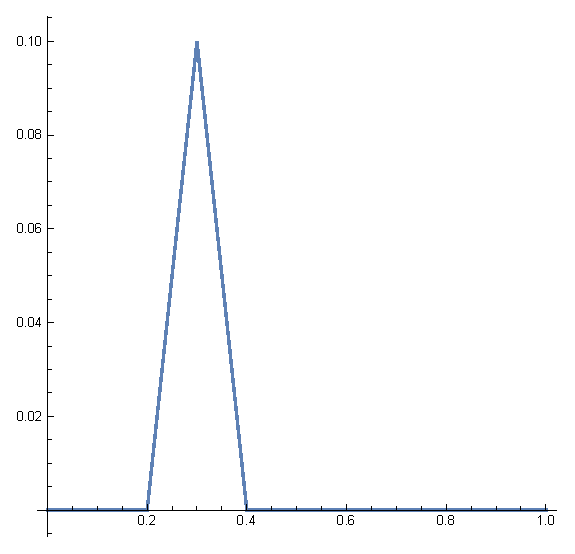
\includegraphics[width=5.5cm]{peak.eps}
\caption{A peak function where $a=0$, $b=1$, $t=0.2$, $h=0.1$. \label{fig:peakfunction}}
\end{figure}
\begin{gather*}
  \text{peak}'(x;t,h):= \begin{cases} \displaystyle 1, & t \le x < t+h,\\[1ex]
\displaystyle -1, & t+h \le x < t+2h,\\[1ex]
\displaystyle  0, & \text{otherwise},
\end{cases}, \\
\Var(\text{peak}'(\cdot;t,h))\le 4 \text{ with equality if } a<t<t+2h<b, \\
\int_{a}^{b}\text{peak}(x;t,h)dx=h^2.
\end{gather*}
The peak function above is continuous and with finite variation of the first derivative of the function shown in \ref{fig:peakp1}:
\begin{figure}[ht]
\centering
\includegraphics[width=5.5cm]{peakp1.eps}
\caption{First derivative of peak function \ref{peakfunction}. \label{fig:peakp1}}
\end{figure}

With this peak function $\text{peak}'(x;t,h)$, we can now build the following double-peak function:
\begin{subequations}
    \begin{multline}\label{foolingfunctiontrap}
        \text{twopk}(x;t,h,\pm):=\text{peak}(x;a,\mathfrak{h})\pm\frac{3[\mathfrak{C}(h)-1]}{4}\text{peak}(x;t,h)\\ a+3\mathfrak{h}\le t \le b-3h, 0\le h <\mathfrak{h}.
    \end{multline}
    \\
    \begin{equation}
        \Var(\text{twopk}'(x;t,h,\pm))=3+4\frac{3[\mathfrak{C}(h)-1]}{4}=3\mathfrak{C}(h).
    \end{equation}
\end{subequations}
Picture \ref{fig:twopkfunction} shows the shape of the double-peak function.
\begin{figure}
\centering
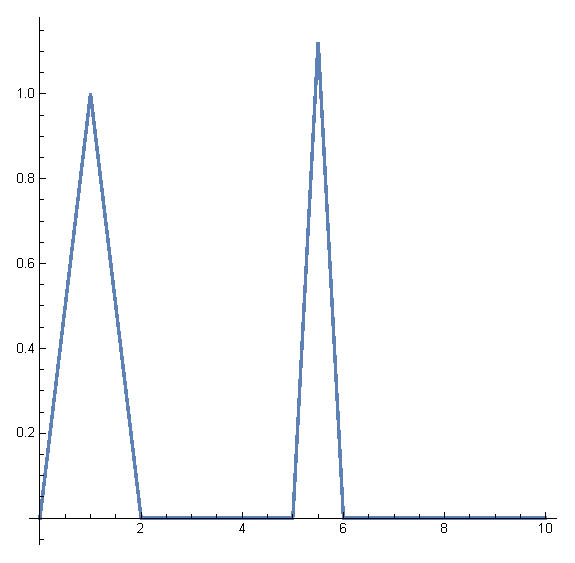
\includegraphics[width=5.5cm]{twopk.eps}
\caption{A fooling function that can fool the trapezoidal rule algorithm, where $a=0$, $b=1$, $t=0.5$, $h=0.05$ and $\mathfrak{h}=0.1$. \label{fig:twopkfunction}}
\end{figure}
Note that $\text{twopk}(x;t,h,\pm)$ are always in $\cc^1$:
From this definition it follows that
\begin{align*}
  &\mathfrak{C}(\text{size}(\{x_j\}_{j=0}^{n+1}))\widehat{V}(\text{twopk}'(x;t,h,\pm),\{x_j\}_{j=0}^{n+1})\\
  \ge & \begin{cases} \displaystyle 3\mathfrak{C}(h)=\Var(\text{twopk}'(x;t,h,\pm)), h \le \text{size}(\{x_j\}_{j=0}^{n+1})) <\mathfrak{h}\\[1ex]
                      \displaystyle \mathfrak{C}(0)\Var(\text{twopk}'''(x;t,h,\pm)), 0\le \text{size}(\{x_j\}_{j=0}^{n+1}))<h
        \end{cases}\\
  \ge & \Var(\text{twopk}'(x;t,h,\pm))
\end{align*}
The functions $\text{twopk}(x;t,h,\pm)$ have two peaks. The first always starts from the left end, $a$, and has the width of $2\mathfrak{h}$. The second will start from any point $t$ that is at least one interval right to the first peak and have a smaller width of $2h$. Although $\text{twopk}(x;t,h,\pm)$ may have a bump with arbitrarily small width $2h$, the height is small enough for $\text{twopk}(x;t,h,\pm)$ to lie in the cone. This function then can be used as our fooling functions.

With the fooling function, we can find the lower bound of complexity of the trapezoidal algorithm. The key to the proof is that, one appropriate $h$ needs to be found such that the smaller peak will reside within one interval of data sites, then cannot be detected by the algorithm. Then, the algorithm cannot distinguish between $\text{peak}'(x;t,h)$ and $\text{twopk}(x;t,h,\pm)$. Assuming that the algorithm $\textup{int}(\cdot,\varepsilon)$ uses $n$ equally spaced nodes to successfully return and answer. Moreover, assuming that $\{x_{j}\}_{j=1}^{m}$ is a subinterval of $\{x_{j}\}_{j=0}^{n}$ where the smaller peak resides. In order to find the proper $h$, notice that average width of intervals is $(x_{m+1}-x_{0})(m+1)$ and $x_{m+1}-x_{0}=b-a-3\mathfrak{h}-h$. Choose one interval such that the width is less than $2h$, the width of small bump. In order to do that, we can choose interval wider than average and $2h$ narrower than average.

  \begin{align*}
    \frac{x_{j+1}-x_{j}}{2}&\ge\frac{x_{m+1}-x_{0}}{2(m+1)}\ge\frac{x_{m+1}-x_{0}}{2(n+1)}=\frac{b-a-3\mathfrak{h}-h}{2n+2}=h,\\
    \Rightarrow h&=\frac{b-a-3\mathfrak{h}}{2n+3}
  \end{align*}

Therefore, the lower bound of the complexity for the integration problem using trapezoidal rule can be represented as:
\begin{theorem} \label{comptrap}
Let $\textup{int}(\cdot,\varepsilon)$ be any (possibly adaptive) algorithm that succeeds for all integrands in $\cc^1$, and only uses function values. For any error tolerance $\varepsilon > 0$ and any arbitrary value of $\Var(f')$, there will be some $f\in \cc^1$ for which $\textup{int}(\cdot,\varepsilon)$ must use at least
    \begin{equation}\label{complowbdtrap}
        -\frac{3}{2}+\frac{b-a-3\mathfrak{h}}{8}\sqrt{\left[\frac{[\mathfrak{C}(0)-1]\Var( f')}{\varepsilon}\right]}
    \end{equation}
    function values. As $\Var(f')/\varepsilon \rightarrow \infty$ the asymptotic rate of increase is the same as the computational cost of Algorithm \ref{multistagetrapalgo}. The adaptive trapezoidal Algorithm \ref{multistagetrapalgo} has optimal order for integration of functions in $\cc^1$.
\end{theorem}
\begin{proof}
  For any positive $\alpha$, suppose that $\textup{int}(\cdot,\varepsilon)$ evaluates integrand $\alpha\text{peak}'(\cdot;t,h)$ at $n$ nodes before returning to an answer. Let $\{x_j\}_{j=1}^{m})$ be the $m<n$ ordered nodes used by $\texttt{int}(\cdot,\varepsilon)$ that fall in the interval $(x_{0},x_{m+1})$ where $x_{0}:=a+2\mathfrak{h}$, $x_{m+1}:=b-h$ and $h:=(b-a-3\mathfrak{h})/(2n+3)$. There must e at least one of these $x_{j}$ with $i=0,\cdots,m$ for which
  \begin{align*}
    \frac{x_{j+1}-x_{j}}{2}\ge\frac{x_{m+1}-x_{0}}{2(m+1)}\ge\frac{x_{m+1}-x_{0}}{2(n+1)}=\frac{b-a-3\mathfrak{h}-h}{2n+2}=h.
  \end{align*}
  Choose one such $x_{j}$ and call it $t$. The choice of $t$ and $h$ ensures that $\textup{int}(\cdot,a,b,\varepsilon)$ cannot distinguish between $\alpha\textup{peak}(\cdot;t,h)$ and $\alpha\textup{twopk}(\cdot;t,h,\pm)$. Thus
  \begin{align*}
    \textup{int}(\alpha\text{twopk}(\cdot;t,h,\pm),a,b,\varepsilon)=\textup{int}(\alpha\text{peak}(\cdot;t,h),a,b,\varepsilon)
  \end{align*}
  Moreover, $\alpha\text{peak}(\cdot;t,h)$ and $\alpha\text{twopk}(\cdot;t,h,\pm)$ are all in the cone $\cc^1$. This means that $\textup{int}(\cdot,\varepsilon)$ is successful for all of the functions.
  \begin{subequations}
  \begin{multline*}
    \varepsilon\ge\frac{1}{2}\left[\right.\left|\int_{a}^{b}\alpha\textup{twopk}(x;t,h,-)dx-\textup{int}(\alpha\textup{twopk}(\cdot;t,h,-),a,b,\varepsilon)\right|\\
    +\left|\int_{a}^{b}\alpha\textup{twopk}(x;t,h,+)dx-\textup{int}(\alpha\textup{twopk}(\cdot;t,h,+),a,b,\varepsilon)\right|\left.\right]
  \end{multline*}
  \begin{multline*}
    \ge\frac{1}{2}\left[\right.\left|\textup{int}(\alpha\textup{peak}(\cdot;t,h,-),a,b,\varepsilon)-\int_{a}^{b}\alpha\textup{twopk}(x;t,h,-)dx\right|\\
    +\left|\int_{a}^{b}\alpha\textup{twopk}(x;t,h,+)dx-\textup{int}(\alpha\textup{peak}(\cdot;t,h,+),a,b,\varepsilon)\right|\left.\right]
  \end{multline*}
  \begin{align*}
     &\ge\frac{1}{2}\left|\int_{a}^{b}\alpha\textup{twopk}(x;t,h,+)dx-\int_{a}^{b}\alpha\textup{twopk}(x;t,h,-)dx\right|\\
     &=\int_{a}^{b}\alpha\textup{peak}(x;t,h)dx\\
     &=\frac{3\alpha[\mathfrak{C}(h)-1]h^2}{4}\\
     &=\frac{[\mathfrak{C}(h)-1]h^2\Var(\alpha\textup{peak}'(\cdot;a,\mathfrak{h}))}{4}
  \end{align*}
  \end{subequations}
  Substituting $h$  in terms of $n$:
      \begin{align*}
        2n+3=\frac{b-a-3\mathfrak{h}}{h}&\ge(b-a-3\mathfrak{h})\left[\frac{[\mathfrak{C}(h)-1]\Var(\alpha \textup{peak}'(\cdot;a,\mathfrak{h})))}{4\varepsilon}\right]^{1/2},\\
        &\ge\frac{b-a-3\mathfrak{h}}{2}\left[\frac{[\mathfrak{C}(0)-1]\Var(\alpha \textup{peak}'(\cdot;a,\mathfrak{h}))}{\varepsilon}\right]^{1/2}.
    \end{align*}
    Since $\alpha$ is an arbitrary positive number, the value of $\Var(\alpha \textup{peak}'(\cdot;a,\mathfrak{h}))$ is arbitrary.

    Finally, comparing the upper bound on the computational cost of $\textup{integral}$ in \eqref{uppbndcostineq} with the lower bound on the computational cost of the best algorithm in \eqref{lowbndcostineq}, both of them increase as $\mathcal{O}((\Var(f')/\varepsilon))^{1/2}$ as $(\Var(f')/\varepsilon)^{1/2}\rightarrow \infty$. Thus $\textup{integral}$ is optimal.
\end{proof}

\Section{Simpson's rule}

To build the fooling functions for Simpson's rule, we will continue our B-Spline expansion in the previous section in order to find the functions the such that $f,f',f''$ are continuous and $\Var(f''')<\infty$.??? Change $f$

\begin{align*}
  \text{b}_{j,0}(x):= \begin{cases} \displaystyle 1, & t_{j} \le x < t_{j+1},\\[1ex]
\displaystyle  0, & \text{otherwise},
\end{cases}
\end{align*}

\begin{align*}
  \text{b}_{j,1}(x):= \begin{cases} \displaystyle \frac{x-t_{j}}{h}, & t_{j} \le x < t_{j+1},\\[1ex]
\displaystyle \frac{t_{j+2}-x}{h}, & t_{j+1} \le x < t_{j+2},\\[1ex]
\displaystyle  0, & \text{otherwise},
\end{cases}
\end{align*}

\begin{align*}
  \text{b}_{j,2}(x):= \begin{cases} \displaystyle \frac{(x-t_{j})^2}{2h^2}, & t_{j} \le x < t_{j+1},\\[1ex]
\displaystyle \frac{(t_{j+2}-x)(x-t_{j})}{2h^2}+\frac{(t_{j+3}-x)(x-t_{j+2})}{2h^2}, & t_{j+1} \le x < t_{j+2},\\[1ex]
\displaystyle \frac{(t_{j+3}-x)^2}{2h^2}, & t_{j+2} \le x < t_{j+3},\\[1ex]
\displaystyle  0, & \text{otherwise},
\end{cases}
\end{align*}

\begin{align*}
  \text{b}_{j,3}(x):= \begin{cases} \displaystyle \frac{(x-t_{j})^3}{6h^3}, & t_{j} \le x < t_{j+1},\\[1ex]
\displaystyle \frac{(t_{j+2}-x)(x-t_{j})^2}{6h^3}+\frac{(t_{j+3}-x)(x-t_{j})(x-t_{j+1})}{6h^3}\\[1ex]\displaystyle\quad+\frac{(t_{j+4}-x)(x-t_{j+1})^2}{6h^3},& t_{j+1} \le x < t_{j+2},\\[1ex]
\displaystyle \frac{(t_{j+3}-x)^2(x-t_{j})}{6h^3}+\frac{(t_{j+4}-x)(t_{j+3}-x)(x-t_{j+1})}{6h^3}\\[1ex]\displaystyle\quad+\frac{(t_{j+4}-x)^2(x-t_{j+2})}{6h^3},& t_{j+2} \le x < t_{j+3},\\[1ex]
\displaystyle \frac{(t_{j+4}-x)^3}{6h^3}, & t_{j+3} \le x < t_{j+4},\\[1ex]
\displaystyle  0, & \text{otherwise},
\end{cases}
\end{align*}

%\begin{align*}
%  \text{b}_{j,3}(x):= \begin{cases} \displaystyle \frac{(x-t_{j})^3}{6h^3}, t_{j} \le x < t_{j+1},\\[10ex]
%\displaystyle \frac{(t_{j+2}-x)(x-t_{j})^2}{6h^3}+\frac{(t_{j+3}-x)(x-t_{j})(x-t_{j+1})}{6h^3}+\frac{(t_{j+4}-x)(x-t_{j+1})^2}{6h^3}, \\[1ex]
%\displaystyle \frac{(t_{j+3}-x)^2(x-t_{j})}{6h^3}+\frac{(t_{j+4}-x)(t_{j+3}-x)(x-t_{j+1})}{6h^3}+\frac{(t_{j+4}-x)^2(x-t_{j+2})}{6h^3}, \\[1ex]
%\displaystyle \frac{(t_{j+4}-x)^3}{6h^3}, t_{j+3} \le x < t_{j+4},\\[1ex]
%\displaystyle  0, \text{otherwise},
%\end{cases}
%\end{align*}

\begin{align*}
  \text{b}_{j,3}'''(x):= \begin{cases} \displaystyle 1//h^3, & t_{j} \le x < t_{j+1},\\[1ex]
\displaystyle -3/h^3, & t_{j+1} \le x < t_{j+2},\\[1ex]
\displaystyle 3/h^3, & t_{j+2} \le x < t_{j+3},\\[1ex]
\displaystyle -1/h^3, & t_{j+3} \le x < t_{j+4},\\[1ex]
\displaystyle  0, & \text{otherwise},
\end{cases},
\end{align*}
The function $\text{b}_{j,3}(x)$ is a bump shaped function that starts at point $t_j$, with the width of $t_{j+4}-t_{j}$ and zero value elsewhere than $t_{j}, t_{j+4}$. Assuming that $\{t_{j}\}_{j=1}^{n}$ is equally space between $(a,b)$, $t_{j+1}-t_{j}=h$, and $t=t_{j}$ . We can define our peak function as

%\begin{gather}
%bump(x;t,h):= \begin{cases} \displaystyle (x-t)^3/6, & t \le x < t+h,\\[1ex]
%\displaystyle [(x-t)^2(t+2h-x)+(x-t)(t+3h-x)(x-t-h)+(t+4h-x)(x-t-h)^2]/6, & t+h \le x < t+2h,\\[1ex]
%\displaystyle [(x-t)(t+3h-x)^2+(t+4h-x)(x-t-h)(t+3h-x)+(t+4h-x)^2(x-t-2h)]/6, & t+2h \le x < t+3h,\\[1ex]
%\displaystyle (t+4h-x)^3/6, & t+3h \le x < t+4h,\\[1ex]
%\displaystyle  0, & \text{otherwise},
%\end{cases}
%\\

\begin{align} \label{bumpfunction}
\text{bump}(x;t,h):= \begin{cases} \displaystyle (x-t)^3/6,  &t \le x < t+h,\\[1ex]
\displaystyle [-3(x-t)^3+12h(x-t)^2-12h^2(x-t)+4h^3]/6,\\[1ex] \displaystyle\quad  &t+h \le x < t+2h,\\[1ex]
\displaystyle [3(x-t)^3-24h(x-t)^2+60h^2(x-t)-44h^3]/6,\\[1ex] \displaystyle\quad  &t+2h \le x < t+3h,\\[1ex]
\displaystyle (t+4h-x)^3/6,  &t+3h \le x < t+4h,\\[1ex]
\displaystyle  0,  &\text{otherwise},
\end{cases}
\end{align}
Picture \ref{fig:bumpfunction} shows the shape of the bump function. The bump function is continuous.
\begin{figure}[ht]
\centering
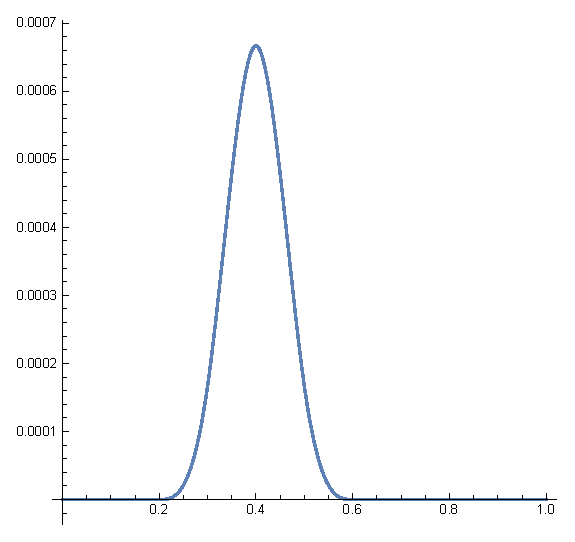
\includegraphics[width=5.5cm]{bump.eps}
\caption{A bump function, where $a=0$, $b=1$, $t=0.2$, $h=0.1$ and $\mathfrak{h}=0.1$. \label{fig:bumpfunction}}
\end{figure}
\begin{subequations}
\begin{gather}
\text{bump}'''(x;t,h):= \begin{cases} \displaystyle 1, & t \le x < t+h,\\[1ex]
\displaystyle -3, & t+h \le x < t+2h,\\[1ex]
\displaystyle 3, & t+2h \le x < t+3h,\\[1ex]
\displaystyle -1, & t+3h \le x < t+4h,\\[1ex]
\displaystyle  0, & \text{otherwise},
\end{cases}, \\
\Var(\text{bump}'''(\cdot;t,h))\le 16 \text{ with equality if } a<t<t+4h<b, \\
\int_{a}^{b}\text{peak}(x;t,h)dx=h^4.
\end{gather}
\end{subequations}
\begin{figure}[ht]
\centering
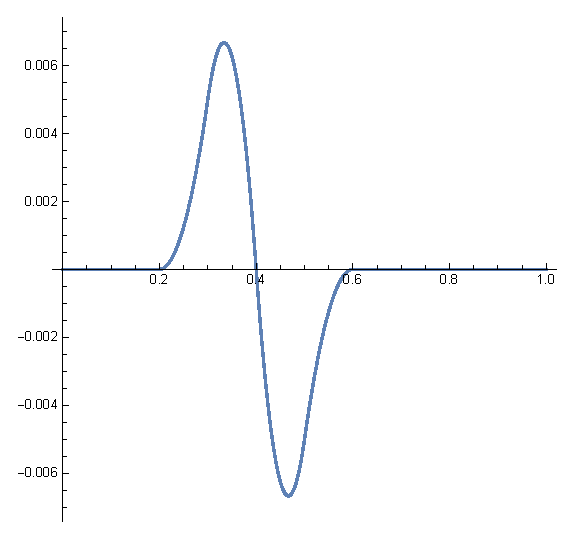
\includegraphics[width=5.5cm]{bumpp1.eps}
\caption{First derivative of bump function. \label{fig:bumpp1}}
\end{figure}
\begin{figure}[ht]
\centering
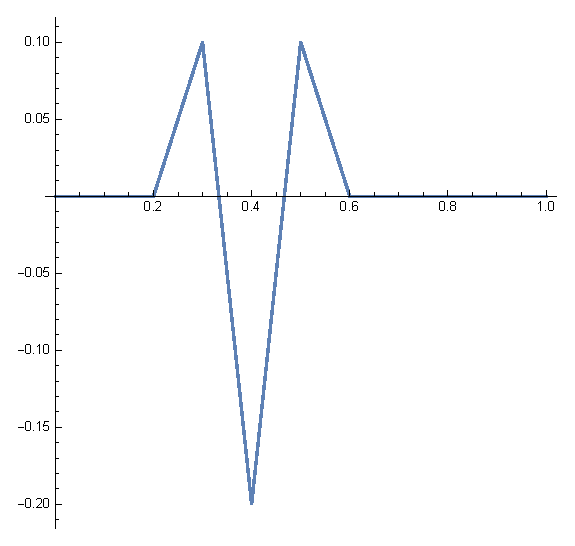
\includegraphics[width=5.5cm]{bumpp2.eps}
\caption{Second derivative of bump function. \label{fig:bumpp2}}
\end{figure}
\begin{figure}[ht]
\centering
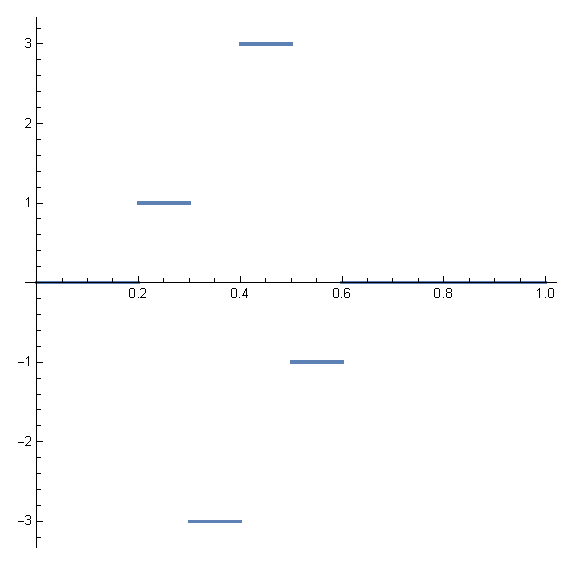
\includegraphics[width=5.5cm]{bumpp3.eps}
\caption{Third derivative of bump function. \label{fig:bumpp3}}
\end{figure}
The bump function above is continuous to the third derivative. We can now build the following double-bump function that is always in $\cc^3$:
\begin{subequations}
    \begin{multline}\label{foolingfunctionsim}
        \text{twobp}(x;t,h,\pm):=\text{bump}(x;a,\mathfrak{h})\pm\frac{15[\mathfrak{C}(h)-1]}{16}\text{bump}(x;t,h)\\ a+5\mathfrak{h}\le h \le b-5h, 0\le h <\mathfrak{h}.
    \end{multline}
    \\
    \begin{equation}
        \Var(\text{twobp}'''(x;t,h,\pm))=15+16\frac{15[\mathfrak{C}(h)-1]}{16}=15\mathfrak{C}(h).
    \end{equation}
\end{subequations}
Picture \ref{fig:twobpfunction} shows the shape of the double-peak function.
\begin{figure}
\centering
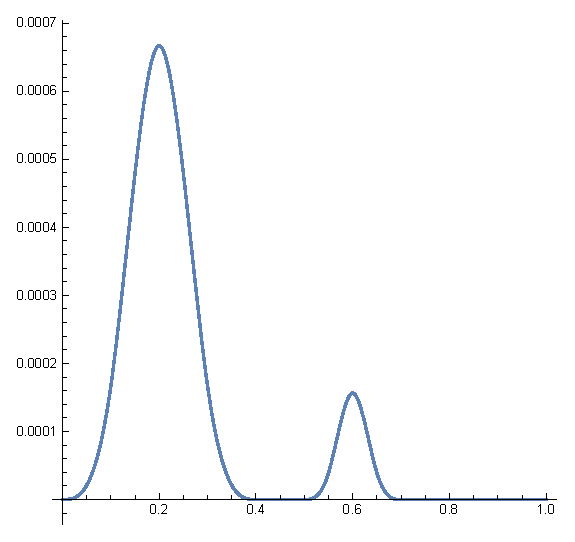
\includegraphics[width=5.5cm]{twobp.eps}
\caption{A fooling function that can fool the Simpson's rule algorithm, where $a=0$, $b=1$, $t=0.5$, $h=0.05$ and $\mathfrak{h}=0.1$. \label{fig:twobpfunction}}
\end{figure}
From this definition it follows that
\begin{align*}
  &\mathfrak{C}(\text{size}(\{x_j\}_{j=0}^{n+1}))\widehat{V}(\text{twobp}'''(x;t,h,\pm),\{x_j\}_{j=0}^{n+1})\\
  \ge & \begin{cases} \displaystyle 15\mathfrak{C}(h)=\Var(\text{twobp}'''(x;t,h,\pm)), h \le \text{size}(\{x_j\}_{j=0}^{n+1})) <\mathfrak{h}\\[1ex]
                      \displaystyle \mathfrak{C}(0)\Var(\text{twobp}'''(x;t,h,\pm)), 0\le \text{size}(\{x_j\}_{j=0}^{n+1}))<h
        \end{cases}\\
  \ge & \Var(\text{twobp}'''(x;t,h,\pm))
\end{align*}
Although $\text{twobp}'''(x;t,h,\pm)$ may have a bump with arbitrarily small width $4h$, the height is small enough for $\text{twobp}'''(x;t,h,\pm)$ to lie in the cone.

Similar to the trapezoidal case, the average width of intervals is $\frac{x_{m+1}-x_{0}}{m+1}$ and $x_{m+1}-x_{0}=b-a-5\mathfrak{h}-h$. Choose one interval such that width less bigger than $4h$ (the width of small bump). In order to do that, we can choose interval wider than average and $4h$ narrower than average:

  \begin{align*}
    \frac{x_{j+1}-x_{j}}{4}&\ge\frac{x_{m+1}-x_{0}}{4(m+1)}\ge\frac{x_{m+1}-x_{0}}{4(n+1)}=\frac{b-a-5\mathfrak{h}-h}{4n+4}=h,\\
    \Rightarrow h&=\frac{b-a-5\mathfrak{h}}{4n+5}
  \end{align*}

With the fooling function, we can find the lower bound of complexity of the Simpson's algorithm.
\begin{theorem}\label{compsim}
    Let $int$ be any (possibly adaptive) algorithm that succeeds for all integrands in $\cc$, and only uses function values. For any error tolerance $\varepsilon > 0$ and any arbitrary value of $\Var(f''')$, there will be some $f\in \cc$ for which $int$ must use at least
    \begin{equation}\label{complowbdsim}
        -\frac{5}{4}+\frac{b-a-5\mathfrak{h}}{8}\left[\frac{[\mathfrak{C}(0)-1]\Var( f''')}{\varepsilon}\right]^{1/4}
    \end{equation}
    function values. As $\Var(f''')/\varepsilon \rightarrow \infty$ the asymptotic rate of increase is the same as the computational cost of Algorithm \ref{multistageintegalgosimpson}. The adaptive Simpson's Algorithm \ref{multistageintegalgosimpson} has optimal order for integration of functions in $\cc^3$.
\end{theorem}
\begin{proof}
  For any positive $\alpha$, suppose that $\texttt{int}(\cdot,\varepsilon)$ evaluates integrand $\alpha\text{bump}'''(\cdot;t,h)$ at $n$ nodes before returning to an answer. Let $\{x_j\}_{j=1}^{m})$ be the $m<n$ ordered nodes used by $\texttt{int}(\cdot,\varepsilon)$ that fall in the interval $(x_{0},x_{m+1})$ where $x_{0}:=a+3\mathfrak{h}$, $x_{m+1}:=b-h$ (why $h$ but not $\mathfrak{h}$ or $5h$?) and $h:=(b-a-5\mathfrak{h})/(4n+5)$. There must e at least one of these $x_{j}$ with $i=0,\cdots,m$ for which
  \begin{align*}
    \frac{x_{j+1}-x_{j}}{4}\ge\frac{x_{m+1}-x_{0}}{4(m+1)}\ge\frac{x_{m+1}-x_{0}}{4(n+1)}=\frac{b-a-5\mathfrak{h}-h}{4n+4}=h.
  \end{align*}
  Choose one such $x_{j}$ and call it $t$. The choice of $t$ and $h$ ensures that $\texttt{int}(\cdot,a,b,\varepsilon)$ cannot distinguish between $\alpha\text{bump}(\cdot;t,h)$ and $\alpha\text{twobp}(\cdot;t,h,\pm)$. Thus
  \begin{align*}
    \texttt{int}(\alpha\text{twobp}(\cdot;t,h,\pm),a,b,\varepsilon)=\texttt{int}(\alpha\text{bump}(\cdot;t,h),a,b,\varepsilon)
  \end{align*}
  Moreover, $\alpha\text{bump}(\cdot;t,h)$ and $\alpha\text{twobp}(\cdot;t,h,\pm)$ are all in the cone $\cc$. This means that $\texttt{int}$ is successful for all of the functions.
  \begin{subequations}
  \begin{multline*}
    \varepsilon\ge\frac{1}{2}\left[\right.\left|\int_{a}^{b}\alpha\text{twobp}(x;t,h,-)dx-\texttt{int}(\alpha\text{twobp}(\cdot;t,h,-),a,b,\varepsilon)\right|\\
    +\left|\int_{a}^{b}\alpha\text{twobp}(x;t,h,+)dx-\texttt{int}(\alpha\text{twobp}(\cdot;t,h,+),a,b,\varepsilon)\right|\left.\right]
  \end{multline*}
  \begin{multline*}
    \ge\frac{1}{2}\left[\right.\left|\texttt{int}(\alpha\text{bump}(\cdot;t,h,-),a,b,\varepsilon)-\int_{a}^{b}\alpha\text{twobp}(x;t,h,-)dx\right|\\
    +\left|\int_{a}^{b}\alpha\text{twobp}(x;t,h,+)dx-\texttt{int}(\alpha\text{bump}(\cdot;t,h,+),a,b,\varepsilon)\right|\left.\right]
  \end{multline*}
  \begin{align*}
     &\ge\frac{1}{2}\left|\int_{a}^{b}\alpha\text{twobp}(x;t,h,+)dx-\int_{a}^{b}\alpha\text{twobp}(x;t,h,-)dx\right|\\
     &=\int_{a}^{b}\alpha\texttt{bump}(x;t,h)dx\\
     &=\frac{15\alpha[\mathfrak{C}(h)-1]h^4}{16}\\
     &=\frac{[\mathfrak{C}(h)-1]h^4\Var(\alpha\texttt{bump}'''(\cdot;a,\mathfrak{h}))}{16}
  \end{align*}
  \end{subequations}
  Substituting $h$  in terms of $n$:
      \begin{align*}
        4n+5=\frac{b-a-5\mathfrak{h}}{h}&\ge(b-a-5\mathfrak{h})\left[\frac{[\mathfrak{C}(h)-1]\Var(\alpha \texttt{bump}'''(\cdot;a,\mathfrak{h})))}{16\varepsilon}\right]^{1/4},\\
        &\ge\frac{b-a-5\mathfrak{h}}{2}\left[\frac{[\mathfrak{C}(0)-1]\Var(\alpha \texttt{bump}'''(\cdot;a,\mathfrak{h}))}{\varepsilon}\right]^{1/4}.
    \end{align*}
    Since $\alpha$ is an arbitrary positive number, the value of $\Var(\alpha \texttt{bump}'''(\cdot;a,\mathfrak{h}))$ is arbitrary.

    Finally, comparing the upper bound on the computational cost of $\texttt{integral}$ in \eqref{uppbndcostineq} with the lower bound on the computational cost of the best algorithm in \eqref{lowbndcostineq}, both of them increase as $\mathcal{O}((\Var(f''')/\varepsilon))^{1/4}$ as $(\Var(f''')/\varepsilon)^{1/4}\rightarrow \infty$. Thus $\texttt{integral}$ is optimal.
\end{proof}


\Chapter{Numerical Experiments}

We use the fooling function \eqref{foolingfunctionsim} to build our test function. Consider the family of bump test functions on interval $(0,1)$ defined by
\begin{equation}\label{testfun}
f(x,t,h)= a\text{twobp}(x;t,h,+)
\end{equation}
with  $t \sim \cu[0.5,1]$, $h \sim \cu[0,1]$, and $a=1/(h^4)$ chosen to make $\int_0^1 f(x) \, \dif x = 1$.
%It follows that $\norm[1]{f'-f(1)+f(0)}=1/a$ and $\Var(f')=2/a^2$.  The probability that $f \in \cc_{\tau}$ is $\min\left(1,\max(0,\left(\log_{10}(\tau/2)-1\right)/3)\right).$

%As an experiment, we chose $10000$ random test functions and applied Algorithm \ref{multistagetrapalgo} and Algorithm \ref{multistageintegalgosimpson} with an error tolerance of  $\varepsilon = 10^{-8}$ and initial $\mahtfrak{h}$ values of $0.1$.  The algorithm is considered successful for a particular $f$ if the exact and approximate integrals agree to within $\varepsilon$. The success and failure rates are given in Table \ref{integresultstable}. Our algorithm imposes a cost budget of $N_{\max}=10^7$.
%If the proposed $n_{i+1}$ in Stages 2 or 3 exceeds $N_{\max}$, then our algorithm returns a warning and falls back to the largest possible $n_{i+1}$ not exceeding $N_{\max}$ for which $n_{i+1}-1$ is a multiple of $n_i-1$.  The probability that $f$ initially lies in $\cc_{\tau}$ is the smaller number in the third column of Table \ref{integresultstable}, while the larger number is the empirical probability that $f$ eventually lies in $\cc_{\tau}$ after possible increases in $\tau$ made by Stage 2 of Algorithm \ref{multistageintegalgo}.  For this experiment Algorithm \ref{multistageintegalgo} was successful for all $f$ that finally lie inside $\cc_{\tau}$ and for which no attempt was made to exceed the cost budget.

\begin{table}[h]
\centering
\begin{tabular}{cccccc}
&&&Success & Success & Failure \\
& $\tau$ &  $\Prob(f \in \cc_{\tau}) $ & No Warning & Warning & No Warning \\
\toprule
&$10$ & $0\% \rightarrow  25\% $ & $25\%$ & $<1\%$ & $75\%$  \\
Algorithm \ref{multistageintegalgo}
 &$100$ & $23 \% \rightarrow 58\% $ & $56\%$ & $2\%$ & $42\%$ \\
&$1000$ & $57\% \rightarrow 88\% $& $68\%$ & $20\%$ &$12\%$ \\
\midrule
{\tt quad} & & & 8\% & & $92\%$\\
{\tt integral} & & & 19\% & & $81\%$\\
{\tt chebfun} & & &29\% & & $71\%$\\
\end{tabular}
\caption{The probability of the test function lying in the cone for the original and eventual values of $\tau$ and the empirical success rate of Algorithm \ref{multistageintegalgo} plus the success rates of other common quadrature algorithms. \label{integresultstable}}
\end{table}

Some commonly available numerical algorithms in MATLAB are {\tt quad} and {\tt integral} \cite{MAT8.1} and the MATLAB Chebfun toolbox \cite{TrefEtal12}. We applied these three routines to the random family of test functions.  Their success and failure rates are also recorded in Table \ref{integresultstable}.  %They do not give warnings of possible failure.

\Section{Simpson's Rule}
\textcolor{red}{I need to use a good example to run the tests. Then I will need to compare the results for both algorithms with other algorithms. After that, I need to compare trap and sim to get the conclusion such as sim has faster convergence rate than trap. This will require an sample function good to both trap and sim.}



\Chapter{CONCLUSION}
 %   \input{Conclusion.tex}

A


\Section{Summary}

A

\clearpage


%
% APPENDIX
%

% Do the settings of appendices with \appendix command
\appendix

% Then create each appendix using
% \Appendix{title_of_appendix} command

\Appendix{Table of Transition Coefficients for the Design of
Linear-Phase FIR Filters}

Your Appendix will go here !

% \moretox

  \Appendix{Name of your Second
Appendix}

Your second appendix text....

\Appendix{Name of your Third Appendix}

Your third appendix text....
%
% BIBLIOGRAPHY
%
% you have two options: 1) create bibliography manually,
% 2) create bibliography automatically. See BibliographyHelp.pdf file for details.

%
\bibliographystyle{plain}
\bibliography{mybib}

\end{document}  % end of document
